\documentclass{article}
\usepackage[T1]{fontenc}
\usepackage{graphicx}
\usepackage {subfigure}
\usepackage{color}
\usepackage{hyperref}
\usepackage{amsmath,amsfonts,amssymb}
\setlength{\parskip}{1em}
\usepackage{scrextend}
\usepackage{lscape}
\usepackage{url}

\title{Projet Maths}
\author{ O. BRIODEAU, C. GOUMENT, A.S. MILEA, B. PALACHEV, D. TOOMEY}
\date{D\'{e}cembre 2016}

\begin{document}

\maketitle

\vspace{10\baselineskip}
\begin{center}
\makeatother
\title{L'INTERPOLATION PAR SPLINE}\\
\end{center}

\vspace{12\baselineskip}
\begin{center}
A l'attention de M.Gleyse\\
\date{2016-2017}
\end{center}

\newpage
\renewcommand{\contentsname}{\begin{center}Sommaire \end{center}}
\tableofcontents

\newpage
\section{Introduction} 

	Depuis toujours, les savants cherchent de meilleures m\'{e}thodes de r\'{e}solution \`{a} l'aide des math\'{e}matiques pour r\'{e}soudre des probl\`{e}mes de calcul et de repr\'{e}sentation graphique les plus courants dans les domaines de l'industrie et des sciences. Un des aspects essentiels de ces domaines est la pr\'{e}cision des mesures et notamment la fid\'{e}lit\'{e} des approximations.
\\
\indent
	Du fait que les \'{e}tudes de la nature ne sont en g\'{e}n\'{e}ral pas mod\'{e}lis\'{e}es par des formules math\'{e}matiques standards, nous nous trouvons alors oblig\'{e}s de passer par des estimations \`{a} l'aide d'op\'{e}rations avec plusieurs fonctions de base. Ces m\'{e}thodes entra\^{i}nent dans la majorit\'{e} des cas des erreurs et des incertitudes plus ou moins importantes. Ainsi, nous nous demandons : comment pourrait-on diminuer ces inexactitudes afin d'obtenir des r\'{e}sultats plus coh\'{e}rents avec la r\'{e}alit\'{e} ?
\\
\indent
	De nos jours, chaque scientifique est confront\'{e} \`{a} tracer et \`{a} \'{e}tudier une courbe exp\'{e}rimentale de la 
fa\c con la plus pertinente possible en partant de l'unique connaissance de quelques points. Il est alors essentiel de donner avec le plus de pr\'{e}cision possible les courbes de tendance et courbes lisses qui relient ces points que ce soit en chimie (courbes ph-m\'{e}triques, graphiques potentiom\'{e}triques), en thermodynamique (courbes d'enthalpies), en \'{e}conomie ou en m\'{e}canique (courbes de r\'{e}sistance des mat\'{e}riaux, etc)
\\
\indent
	La plupart des domaines scientifiques ou industriels requi\`{e}rent la meilleure pr\'{e}cision d'approximation de courbe afin de trouver des r\'{e}sultats exp\'{e}rimentaux qui sont bien en accord avec la r\'{e}alit\'{e}. Aujourd'hui, un des algorithmes les plus efficaces utilis\'{e}s pour l'\'{e}tude et la repr\'{e}sentation des courbes est l'interpolation num\'{e}rique.
\\
\indent
	D'apr\`{e}s le dictionnaire Larousse, l'interpolation est \guillemotleft l'op\'{e}ration consistant \`{a} d\'{e}terminer, \`{a} partir d'une s\'{e}rie statistique succincte aux valeurs trop espac\'{e}es, de nouvelles valeurs correspondant \`{a} un caract\`{e}re interm\'{e}diaire pour lequel aucune mesure n'a \'{e}t\'{e} effectu\'{e}e \guillemotright. Ce terme est employ\'{e} dans plusieurs domaines avec des significations vari\'{e}es :
\\
- en philologie (\'{e}tude critique de textes), une interpolation est un extrait de texte introduit dans une \oe{}uvre \`{a} laquelle il n'appartient pas ;
\\
- en imagerie num\'{e}rique l'interpolation consiste \`{a} redimensionner l'image en diminuant ou en
augmentant la matrice de l'image initiale, et donc le nombre de pixels ;
\\
- en musique, une interpolation permet d'obtenir une valeur de note ou de rythme situ\'{e}e entre deux
valeurs connues ;
\\
- dans l'industrie des films et d'animation, le principe d'interpolation est connu sous le nom de \guillemotleft Tweening \guillemotright, un proc\'{e}d\'{e} qui permet de cr\'{e}er des images interm\'{e}diaires successives de telle sorte qu'une image s'encha\^{i}ne agr\'{e}ablement et de fa\c con fluide avec la suivante ;
\\
- en m\'{e}thodologie, l'interpolation est le rapprochement d'une situation avec des situations-type ou
mod\`{e}les ;
\\
- en informatique, une interpolation permet l'\'{e}valuation de variables ou d'expressions \`{a} l'int\'{e}rieur
d'une cha\^{i}ne de caract\`{e}res litt\'{e}rale (par exemple Perl 6 est particuli\`{e}rement riche en convention
d'interpolation) ;
\\
- en math\'{e}matiques : l'interpolation est une op\'{e}ration permettant de construire une courbe \`{a} partir de fonctions, elles-m\^{e}mes trouv\'{e}es \`{a} partir d'un nombre fini de points donn\'{e}s ;
\par
Dans ce rapport, nous nous concentrerons uniquement sur le domaine des math\'{e}matiques. Plus pr\'{e}cis\'{e}ment, nous nous int\'{e}resserons \`{a} la technique de construction de courbes gr\^{a}ce aux fonctions qu'on \'{e}tablira \`{a} partir d'un nombre donn\'{e} de points et des conditions initiales du probl\`{e}me.
\par
	En math\'{e}matique, on peut distinguer plusieurs m\'{e}thodes d'interpolation :
\\
- l'interpolation lin\'{e}aire : on constitue une courbe d'interpolation qui est une succession de segments, \`{a} savoir relier des points entre eux par des portions de droites ;
\\
- l'interpolation polynomiale, consiste \`{a} utiliser un polyn\^{o}me unique et non des tron\c cons, de degr\'{e}s aussi grands que n\'{e}cessaire, pour estimer localement l'\'{e}quation repr\'{e}sentant la courbe, afin de d\'{e}terminer la valeur entre les \'{e}chantillons \`{a} l'aide de la m\'{e}thode de d\'{e}termination lagrangienne, la m\'{e}thode plus d\'{e}velopp\'{e}e d'interpolation d'Hermite ou gr\^{a}ce aux diff\'{e}rences finies de Newton ;
\\
- l'interpolation par cosinus : on applique la fonction cosinus en deux points fix\'{e}s pour mod\'{e}liser localement la courbe. La tangente \`{a} chaque pic est horizontale, ce qui signifie que chaque pic de la fonction correspond r\'{e}ellement \`{a} un point connu de la courbe discr\`{e}te ;
\\
- l'interpolation cubique : on utilise une \'{e}quation cubique pour mod\'{e}liser localement la courbe et on \'{e}value la fonction en quatre points qui remplace la courbe discr\`{e}te. Concernant les conditions de continuit\'{e}, la forme de la cubique peut varier et donner une interpolation diff\'{e}rente (interpolation cubique de Keys ou interpolation par spline cubique). La tangente en chaque point d'indice i poss\`{e}de la m\^{e}me pente que le segment reliant les points d'indice $-1$ et $i+1$, ce qui signifie que chaque pic de la courbe peut \^{e}tre d\'{e}pass\'{e} par la courbe interpol\'{e}e ;
\par
	Nous pouvons d\'{e}finir le terme spline par une fonction polynomiale d\'{e}finie par morceaux avec diff\'{e}rents polyn\^{o}mes sur chaque intervalle. Ainsi, une interpolation par spline est obtenue par l'assemblage de plusieurs polyn\^{o}mes de faibles degr\'{e}s en des points donn\'{e}s. Notre but principal est de pr\'{e}senter la sp\'{e}cificit\'{e} et la m\'{e}thodologie de l'interpolation par spline cubique. De ce fait, nous consid\'{e}rons les conditions de continuit\'{e} sp\'{e}cifiques \`{a} cette technique.
\\
\indent
	Il existe \'{e}galement d'autres proc\'{e}d\'{e}s pour \'{e}tudier et tracer des courbes. Les courbes de B\'{e}zier et les B-splines sont des m\'{e}thodes parmi les plus efficaces. Elles sont habituellement utilis\'{e}es pour la mod\'{e}lisation de surfaces complexes sur des logiciels informatiques de mod\'{e}lisation de type CAO (Conception Assist\'{e}e par Ordinateur). Dans ce rapport, nous allons aussi pr\'{e}senter dans leur aspect g\'{e}n\'{e}ral ces deux techniques avec leurs points forts et leurs points faibles.

\subsection{Formulation du probl\`{e}me}

	Soient des points $A_i$ quelconques de coordonn\'{e}es $(x_i , y_i )$, $i = 0, …,n$ . La m\'{e}thode d'interpolation par spline cubique consiste \`{a} trouver une fonction $s(x)$ d\'{e}finie sur un intervalle I = [a; b] d\'{e}finie sur $\mathbb{R}$ tel que:
\\
- cette fonction relie chaque points $A_i $ et $A_{ i+1}$ par une spline cubique (polyn\^{o}me de degr\'{e}s 3 maximum) avec n indices naturels ;
\\
- chaque spline est de classe $C^2$ (deux fois d\'{e}rivables avec les d\'{e}riv\'{e}es d'ordre 1 et 2 continues) en tout point $A_i$. La classe $C^2$ est une condition n\'{e}cessaire pour l'interpolation par spline cubique.
\par    
	On se demande alors comment utiliser l'interpolation par spline cubique pour tracer une courbe.
\\
\indent
	Afin de r\'{e}pondre \`{a} cette question, nous aborderons le probl\`{e}me d'un point de vue math\'{e}matique puis informatique. Nous verrons ainsi par des d\'{e}monstrations, des exemples, et par l'interm\'{e}diaire de deux programmes (un pour les splines cubiques, l'autre pour les B-splines), comment obtenir une fonction spline cubique. Enfin, nous tenterons de cerner les diff\'{e}rents enjeux scientifiques et industriels de cette m\'{e}thode.

\subsection{Point Historique}

	D\'{e}couvrir et innover n\'{e}cessitent une certaine distanciation par rapport \`{a} notre pass\'{e} et pr\'{e}sent. Il reste cependant n\'{e}cessaire de s'inspirer des grandes d\'{e}couvertes qui sont venues auparavant. Comprendre le contexte de l'utilisation de cet outil math\'{e}matique constitue un int\'{e}r\^{e}t important pour r\'{e}ussir \`{a} nous placer dans le c\oe{}ur du sujet et comprendre toutes les influences fondatrices et, l'\'{e}volution de la fa\c con de r\'{e}soudre notre probl\`{e}me. En effet, comme le disait Leibniz, \guillemotleft C'est une chose extr\^{e}mement utile que d'avoir connaissance de l'origine v\'{e}ritable de d\'{e}couvertes m\'{e}morables, et en particulier de celles qui ont \'{e}t\'{e} faites sciemment et par r\'{e}flexion, et non par chance \guillemotright. C'est pour cela qu'il est int\'{e}ressant de conna\^{i}tre l'histoire et le d\'{e}veloppement d'un champ auquel on s'int\'{e}resse.
\par
	Dans le cadre de ce projet il est essentiel de pr\'{e}senter \`{a} la fois les origines de l'interpolation en g\'{e}n\'{e}rale et notamment la naissance et l'utilisation des splines au cours du temps.

\subsubsection{Les origines de l'interpolation}

	L'interpolation comme outil math\'{e}matique n'est pas un concept nouveau. En effet, on retrouve des exemples d'utilisation tr\`{e}s t\^{o}t dans l'histoire de l'Homme. Ses premi\`{e}res applications ont principalement eu lieu dans le domaine de l'astronomie. En effet, les astronomes Babyloniens sont r\'{e}put\'{e}s pour avoir utilis\'{e} l'interpolation lin\'{e}aire et polynomiale de degr\'{e}s \'{e}lev\'{e}s aux alentours de 300 av. JC afin de pr\'{e}voir les positions des astres dans les \'{e}ph\'{e}m\'{e}rides (ouvrage qui contient les positions des astres \`{a} des moments donn\'{e}s). Par ailleurs, quelques tables de pierre montrent aussi des techniques d'interpolation complexe. Malheureusement, la plupart de ces recherches se sont trop d\'{e}grad\'{e}es au cours de temps.

\begin{figure}[h]
	\centering
	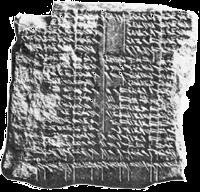
\includegraphics[width=4cm]{cuneiform.jpg}
	\caption{Ancienne table de pierre}
\end{figure}

\indent
	Puis en 150 av. JC, Hipparque, un astronome grec, utilise \`{a} son tour l'interpolation lin\'{e}aire afin de rassembler ses tables de cordes, une sorte de table trigonom\'{e}trique primitive afin de pr\'{e}voir les trajets de la lune et du soleil et les positions des corps c\'{e}lestes.
\\
\indent
	En 160 apr\`{e}s JC, Claudius Ptolemy, un astronome math\'{e}maticien grec d'origine \'{e}gyptienne, utilise des tables contenant une grande diversit\'{e} de fonctions trigonom\'{e}triques pour d\'{e}crire l'univers d'un point de vue g\'{e}ocentrique. Pour \'{e}viter les calculs incommodes, il utilise une interpolation lin\'{e}aire adapt\'{e}e avec deux bornes pour trouver les valeurs interm\'{e}diaires de tableaux. Il est \`{a} l'origine de Almagest (\guillemotleft La compilation math\'{e}matique\guillemotright). C'est un ouvrage contenant les connaissances les plus avanc\'{e}es de l'Antiquit\'{e} dans les domaines des math\'{e}matiques et de l'astronomie.
\\
\indent
	Plus tard, entre 600 et 800 apr\`{e}s JC, les chinois et les indiens d\'{e}veloppent chacun de leur c\^{o}t\'{e} l'interpolation du deuxi\`{e}me ordre. Ces d\'{e}couvertes correspondent \`{a} des versions \'{e}quivalentes aux formules de Gregory-Newton et Newton-Gauss pour des intervalles in\'{e}gaux trouv\'{e}es aux XIII\`{e}me si\`{e}cle.
\\
\indent
	En l'an 1000, le scientifique arabe al-Biruni \'{e}crit une \oe{}uvre sur l'interpolation d'ordre 2 en reprenant quelques donn\'{e}es des recherches indiennes et presque 300 ans plus tard, les chinois mettent en place les bases de l'interpolation d'ordre 3. On remarque en particulier le math\'{e}maticien Zhu Shijie qui \'{e}crit en 1303 son \oe{}uvre majeure. Il effectue des recherches tr\`{e}s innovatrices concernant l'interpolation et trouve une solution proche de la formule de Gregory-Newton. 
Malgr\'{e} tout, toutes ces m\'{e}thodes donnent des r\'{e}sultats avec une pr\'{e}cision trop faible. Il faudra attendre 1611 pour la d\'{e}couverte d'Harriot, un math\'{e}maticien anglais. Celle-ci consiste en une m\'{e}thode d'interpolation pr\'{e}cise qui va jusqu'aux diff\'{e}rences d'ordre cinq. Sa m\'{e}thode est consid\'{e}r\'{e}e comme le plus ancien exemple du monde occidental qui utilise les techniques d'interpolation. Quelques ann\'{e}es plus tard, Briggs poursuit le travail de Napier et d\'{e}crit quelques cas particuliers en consid\'{e}rant les diff\'{e}rences d'ordres sup\'{e}rieures ou \'{e}gales \`{a} trois \'{e}tant \'{e}gales \`{a} z\'{e}ro.
\par
	Le mot \guillemotleft interpolation\guillemotright\ appara\^{i}t \`{a} cette p\'{e}riode dans le domaine des math\'{e}matiques. Le math\'{e}maticien John Wallis en est \`{a} l'origine dans son ouvrage en latin, Arithmetica Infinitorum, publi\'{e} en 1655.
\\
\indent
	Dans la lettre adress\'{e}e \`{a} Collins (secr\'{e}taire de la Royal Society), dat\'{e}e du 23 novembre 1670, Gregory \'{e}crit explicitement la fameuse formule d'Interpolation Gregory-Newton. En effet, un des math\'{e}maticiens les plus importants dans le domaine de l'interpolation est Isaac Newton. Son enthousiasme pour ce sujet, quelques formules et concepts th\'{e}oriques peuvent \^{e}tre observ\'{e}s dans les lettres pour Smith et Oldenburg.
\par
	A partir de 1711, Isaac Newton commence \`{a} publier son travail sur l'interpolation en plusieurs livres et manuscrits. Stirling est le premier \`{a} s'int\'{e}resser aux techniques newtoniennes. Ainsi, en 1730, il publie un livre o\`{u} il d\'{e}taille la m\'{e}thode Stirling-Newton.
\\
\indent
	Le comte de Lagrange s'est pench\'{e} sur le probl\`{e}me de l'interpolation au XVIII\`{e}me si\`{e}cle mais il faut attendre l'arriv\'{e}e des ordinateurs pour que le domaine se d\'{e}veloppe r\'{e}ellement. Un aspect tr\`{e}s int\'{e}ressant de sa th\'{e}orie de 1795 \'{e}tait d\'{e}j\`{a} trouv\'{e} par Waring et Euler seize ann\'{e}es plus t\^{o}t, mais la formule est tout de m\^{e}me connue sous le nom de Lagrange.
\\
\indent
	Au XVIII\`{e}me si\`{e}cle, l'interpolation et les approximations servent surtout \`{a} relier ou \`{a} approcher des mesures dans un but scientifique. Avec la r\'{e}volution industrielle, les machines font leur apparition et il faut faire la conception des pi\`{e}ces pour pouvoir les fabriquer. Pour tracer des courbes, les dessinateurs utilisent des m\'{e}thodes manuelles qui reposent sur la d\'{e}formation de lames de m\'{e}tal, de ressorts, l'utilisation de pistolets \`{a} colle et des feuilles de graphiques \`{a} l'\'{e}chelle r\'{e}elle. Pour les surfaces, des gabarits sont construits manuellement en trois dimensions.
\par
	Le XIX\`{e}me si\`{e}cle est plus marqu\'{e} par des \'{e}volutions et juste quelques innovations de la m\'{e}thode d'interpolation. Tout d'abord Gauss, Bessel et Cauchy font des recherches sur le sujet, mais uniquement le math\'{e}maticien fran\c cais trouve une nouvelle formule appel\'{e} le reste de Cauchy. Vers la fin de ce si\`{e}cle, Tchebychef et Hermite innovent la recherche des polyn\^{o}mes d'interpolation et ensuite Weierstrass d\'{e}montre le th\'{e}or\`{e}me d'approximation qui dit que chaque intervalle peut \^{e}tre approxim\'{e} par un polyn\^{o}me, ce qui justifie leur utilit\'{e} pour l'interpolation.
\par   
	L'\'{e}poque moderne est fortement marqu\'{e}e par le d\'{e}veloppement de la technologie et de la communication. Ainsi, de nombreux livres et ouvrages concernant l'interpolation par spline ont \'{e}t\'{e} publi\'{e}s. De plus, du fait que les domaines scientifiques soient en plein essor, l'interpolation commence \`{a} \^{e}tre utilis\'{e}e dans des \'{e}tudes et exp\'{e}riences de plus en plus vari\'{e}es, ce qui entra\^{i}ne l'\'{e}volution des techniques, notamment dans le domaine de l'informatique vers la fin du XX\`{e}me si\`{e}cle.
\\
\indent
	En 1915, E.T.Whittaker d\'{e}veloppe la formule de Newton-Gauss pour un nombre infini d'abscisses \'{e}quidistantes des deux c\^{o}t\'{e}s d'un point donn\'{e} et montre que dans certaines conditions, la fonction de la courbe r\'{e}sultante converge vers la fonction qu'il appelle \guillemotleft $\;$la fonction cardinal\guillemotleft $\;$ qui est une combinaison lin\'{e}aire des fonctions d\'{e}cal\'{e}es sous la forme sin(x)/x. Apr\`{e}s cette d\'{e}couverte, l'accent est mis sur le d\'{e}veloppement de l'interpolation oscillatoire. 
\\
\indent
	A la fin des ann\'{e}es 1940 Shanon et Schoenberg forment une th\'{e}orie novatrice en consid\'{e}rant les fonctions d'interpolation comme des combinaisons lin\'{e}aires de fonctions de base ou des noyaux. Au cours des ann\'{e}es qui suivent, cette nouvelle approche est de plus en plus utilis\'{e}e puis am\'{e}lior\'{e}e et de nouvelles techniques d'interpolation sont exploit\'{e}es et d\'{e}velopp\'{e}es.
\\
\indent
	Toutefois, apr\`{e}s l'apparition des splines, les scientifiques se rendent compte que ces fonctions ont de meilleures propri\'{e}t\'{e}s pour l'interpolation, ce qui permet aux scientifiques d'\'{e}voluer et de perfectionner ces nouvelles m\'{e}thodes de r\'{e}solution.
\\
\indent
	En effet, en 1978 l'utilisation des splines dans les images digitales est r\'{e}volutionn\'{e}e par Hou \& Andrews qui d\'{e}montre la sup\'{e}riorit\'{e} absolue de l'interpolation par B-spline. En outre, des \'{e}tudes r\'{e}centes mettent en exergue l'avantage des splines dans le domaine de l'\'{e}conomie. On remarque que la meilleure pr\'{e}cision d'interpolation est obtenue en utilisant les grains dits O-MOMS r\'{e}cemment introduits par Blu et ses collaborateurs en 2001.
\\
\indent
	Par la suite, nous allons pr\'{e}senter la gen\`{e}se des splines dans le but de comprendre leur \'{e}volution et pourquoi l'on consid\`{e}re que c'est le meilleur outil pour l'interpolation.

\subsubsection{L'interpolation par splines}

	Avant l'invention des ordinateurs, tous les calculs \'{e}taient effectu\'{e}s \`{a} la main. Les fonctions et les fonctions par morceaux sont utilis\'{e}es mais habituellement les polyn\^{o}mes sont adopt\'{e}s du fait de leur facilit\'{e} de manipulation. \`{A} l'origine, le concept de spline est d\'{e}velopp\'{e} pour l'\'{e}laboration et la fabrication de diff\'{e}rentes structures pour les bateaux avant que la mod\'{e}lisation digitale soit impl\'{e}ment\'{e}e \`{a} large \'{e}chelle.
\\
\indent
	D\`{e}s l'apparition des ordinateurs, les splines remplacent les polyn\^{o}mes dans les probl\`{e}mes d'interpolation et par la suite, elles sont exploit\'{e}es dans le cadre de la construction des formes lisses et flexibles aussi au niveau des repr\'{e}sentations graphiques num\'{e}riques. Initialement, le mot \guillemotleft $\;$spline \guillemotright$\;$est utilis\'{e} pour une lamelle mince en m\'{e}tal ou en bois dans le dialecte des anglais de l'est de l'Angleterre.
\\
\indent
	Ensuite, en 1895, la signification change et le mot est employ\'{e} en particulier dans les industries de construction de bateaux et d'avions pour d\'{e}signer la r\`{e}gle flexible utilis\'{e}e pour tracer des courbes sur papier.
\\
\indent
	Pendant de nombreuses ann\'{e}es, les concepteurs de bateaux ont utilis\'{e} des mod\`{e}les r\'{e}duits pour la conception de coques. Le meilleure mod\`{e}le \'{e}tait ensuite dessin\'{e} sur du papier graphique et les points cl\'{e}s de la courbe \'{e}taient plac\'{e}s sur un papier graphique \`{a} \'{e}chelle r\'{e}elle. Une bande en bois \'{e}tait ensuite utilis\'{e}e pour interpoler les points cl\'{e}s par des courbes lisses.
\\
\indent
	L'op\'{e}ration est simple : des bandes en bois (ou compos\'{e}es d'autres mat\'{e}riaux) sont fix\'{e}es au niveau des points cl\'{e}s par des poids en plomb (nomm\'{e}s \guillemotleft$\;$ducks \guillemotright, \guillemotleft $\;$dogs \guillemotright$\;$ou \guillemotleft $\;$rats \guillemotright$\;$en langage technique) et entre ces points, les \'{e}nergies de tension sont calcul\'{e}es de sorte qu'elles soient minimales selon le mat\'{e}riel utilis\'{e} pour la fabrication.
\par
	En 1987, Bartels et Robin Forrest d\'{e}crivent le terme \guillemotleft $\;$ lofting \guillemotright$\;$comme \'{e}tant une technique utilis\'{e}e pendant la deuxi\`{e}me guerre mondiale par l'industrie britannique de construction des avions militaires pour fabriquer des mod\`{e}les pour le fuselage en reliant des bandes minces (nomm\'{e}es splines) \`{a} travers des points cl\'{e}s choisis pr\'{e}alablement et dispos\'{e}es sur un plancher d'un grand loft de design. Un des avions les plus l\'{e}gendaires utilis\'{e}s pendant cette p\'{e}riode qui a r\'{e}volutionn\'{e} la strat\'{e}gie de construction de ces machines est le fameux Spitfire, cr\'{e}\'{e} en utilisant la technique de \guillemotleft $\;$lofting\guillemotleft $\;$. L'entreprise Bristol Aeroplane Company a notamment utilis\'{e} cette technique avec des splines pour produire leurs premiers mod\`{e}les. 
\\
\indent
	Les splines sont apparus nettement apr\`{e}s le th\'{e}or\`{e}me d'\'{e}chantillonnage de Shannon qui s'int\'{e}resse \`{a} la quantit\'{e} d'information contenue ou d\'{e}livr\'{e}e par une source.
	Les premi\`{e}res r\'{e}f\'{e}rences math\'{e}matiques au concept de spline sont associ\'{e}es au math\'{e}maticien Isaac Schoenberg qui pose les bases de ce terme lorsqu'il est employ\'{e} par l'arm\'{e}e am\'{e}ricaine durant la deuxi\`{e}me guerre mondiale.
\\
\indent
	En 1946, Isaac Schoenberg est le premier a utilis\'{e} ce terme dans ses recherches concernant une approximation polynomiale lisse par morceaux. Il a montr\'{e} comment utiliser les splines pour interpoler des \'{e}chantillons \'{e}quidistants pour une fonction. Cependant, Robin Forrest explique qu'une grande difficult\'{e} peut appara\^{i}tre lorsque l'avion est frapp\'{e} par une bombe lanc\'{e} par l'opposition puisque la structure est susceptible de perdre de nombreux composants vitaux \`{a} cause de la faible rigidit\'{e}. De ce fait, ils d\'{e}veloppent une autre m\'{e}thode de fabrication nomm\'{e} \guillemotleft $\;$ conic lofting \guillemotright qui utilise des sections coniques pour mod\'{e}liser les positions des courbes qui se trouvent entre les points cl\'{e}s fix\'{e}s par les dispositifs \guillemotleft $\;$ducks \guillemotright.

\begin{figure}[h]
	\centering
	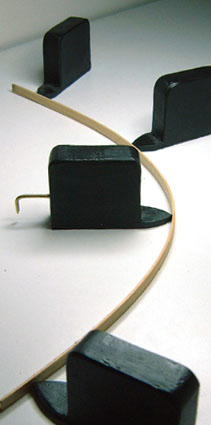
\includegraphics[width=3cm]{ducks.jpg}
	\caption{Ducks}
\end{figure}

\indent
	Isaac Schoenberg a aussi introduit les B-splines, \'{e}l\'{e}ments n\'{e}cessaires \`{a} la construction de splines polynomiaux, mais ces techniques ne sont utilis\'{e}es qu'\`{a} partir des ann\'{e}es 60. Les B-splines remplacent le \guillemotleft $\;$conic lofting \guillemotright quand J. C. Ferguson, employ\'{e} de Boeing, et plus tard, M. A. Sabin, employ\'{e} de British Aircraft Corporation, r\'{e}alisent que ces fonctions peuvent mod\'{e}liser le processus physique de lissage de courbes.
\par
	En ce qui concerne l'utilisation des splines pour la conception et la mod\'{e}lisation des automobiles, on se rend compte que plusieurs projets ind\'{e}pendants sont majoritairement d\'{e}velopp\'{e}s par des chercheurs pour des entreprises de ce milieu pendant la fin des ann\'{e}es 50 et d\'{e}but des ann\'{e}es 60. Ce fait s'explique par la forte concurrence des grands constructeurs automobiles.
\\
\indent
	Ces chercheurs ont pos\'{e} les bases des algorithmes et des techniques pour \'{e}valuer les calculs des courbes. Paul de Casteljau, physicien et math\'{e}maticien de Citro\"{e}n, a d\'{e}velopp\'{e} sa propre analyse num\'{e}rique. Pierre B\'{e}zier, ing\'{e}nieur français en m\'{e}canique et en \'{e}lectricit\'{e} de Renault, a am\'{e}lior\'{e} le travail de Casteljau et a cr\'{e}\'{e} les fameuses Courbes de B\'{e}zier, Birkhoff (qui a \'{e}galement \'{e}tudi\'{e} les probl\`{e}mes d'interpolation en g\'{e}n\'{e}ral) et finalement Garabedian et Boor de General Motors qui ont enrichi le sujet avec des th\'{e}or\`{e}mes et des programmes num\'{e}riques pour la production de voitures.
\\
\indent
	Une seule recherche de Paul de Casteljau n'a \'{e}t\'{e} publi\'{e} en 1959. Cependant, les travaux de Boor de General Motors ont \'{e}t\'{e} publi\'{e} au d\'{e}but des ann\'{e}es 1960, incluant quelques th\'{e}ories fondamentales sur les B-splines. Les r\'{e}sultats du travail fait chez General Motors ont \'{e}t\'{e} d\'{e}taill\'{e} dans les ouvrages de Birkhoff en 1990 et ensuite dans l'ouvrage de Young en 1997. De plus, en 1997, Davis r\'{e}sume toutes ces recherches th\'{e}oriques.
\\
\indent
	Par ailleurs, chez Pratt \& Whitney Aircraft, deux auteurs du premier livre de traitement des splines (Albert et ses collaborateurs en 1967) sont employ\'{e}s pour travailler sur ce sujet. Parall\`{e}lement, Feodor Theilheimer travaille chez David Taylor Model Basin pour augmenter l'utilit\'{e} des splines. 
\par
	Pour am\'{e}liorer la mani\`{e}re de travailler avec les splines, depuis le d\'{e}but des splines, diff\'{e}rents scientifiques, math\'{e}maticiens et ing\'{e}nieurs ont tent\'{e} de trouver d'autres conditions et particularit\'{e}s afin d'obtenir une meilleure pr\'{e}cision. Par exemple, Whittaker a d\'{e}riv\'{e} une spline pour obtenir des donn\'{e}es sur le lissage. Il est le premier \`{a} proposer d'introduire une mesure d'ajustement avec un terme de p\'{e}nalit\'{e} construit \`{a} partir des sommes des carr\'{e}s de la troisi\`{e}me diff\'{e}rence de la fonction pour am\'{e}liorer l'uniformit\'{e} des solutions. En fait, il traite le terme de p\'{e}nalit\'{e} comme une distribution pr\'{e}alable puis il estime les allures et la construction des splines gr\^{a}ce au th\'{e}or\`{e}me de Bayes.
\par
	Le d\'{e}veloppement des splines reste tout de m\^{e}me majoritairement allou\'{e} \`{a} B\'{e}zier. En effet, il a \'{e}t\'{e} le premier \`{a} publier ses r\'{e}sultats lorsque Renault lui en a autoris\'{e}. La recherche sur les splines ne s'en est cependant pas arr\^{e}t\'{e}e l\`{a} et des \'{e}quipes telles que le Biomedical Imaging Group de l'EPFL continuent \`{a} faire progresser le domaine.
\\
\indent
	De nos jours, les splines sont un outil indispensable pour des nombreux domaines allant de la conception des automobiles jusqu'au traitement des sons et le domaine m\'{e}dical.
\\
\indent
	Finalement, de nombreuses \'{e}tudes conduisent \`{a} la conclusion que les splines offrent g\'{e}n\'{e}ralement le meilleur compromis co\^{u}ts-performances. Gr\^{a}ce \`{a} l'\'{e}volution de la technologie, l'interpolation par spline continue \`{a} \^{e}tre am\'{e}lior\'{e}e et les m\'{e}thodes de manipulation \'{e}voluent dans le but d'atteindre la meilleur approximation lorsque l'on \'{e}tudie des probl\`{e}mes de la vie r\'{e}elle.

\newpage
\section{Courbes de B\'{e}zier} 
\subsection{Contexte}

	Dans le cadre de la fabrication des automobiles la mod\'{e}lisation des courbes est une \'{e}tape
fondamentale qui s'est d\'{e}velopp\'{e} notamment pendant l'\'{e}volution de la technologie num\'{e}rique, les ordinateurs en particulier. Pierre B\'{e}zier est un des ing\'{e}nieurs fran\c cais les plus importants qui a d\'{e}di\'{e} sa carri\`{e}re \`{a} la cr\'{e}ation d'un moyen simple et puissant pour mod\'{e}liser des formes et faciliter la programmation des machines \`{a} commande num\'{e}rique afin de rendre la production plus efficace.
\\
\indent
Dipl\^{o}m\'{e} de l'\'{e}cole Nationale Sup\'{e}rieure d'Arts et M\'{e}tiers et de l'\'{e}cole sup\'{e}rieure d'\'{e}lectricit\'{e}, \'{e}l\`{e}ve exceptionnel n\'{e} \`{a} Paris en septembre 1910, Pierre B\'{e}zier entre chez Renault en 1933 o\`{u} il y fera toute sa carri\`{e}re jusqu'en 1975 au poste de directeur des m\'{e}thodes m\'{e}caniques.
Par la suite, d\^{u} \`{a} des divergences avec ses sup\'{e}rieurs, il est mis \`{a} l'\'{e}cart. Cela lui donne l'occasion de s'int\'{e}resser \`{a} un domaine encore presque vierge : la mod\'{e}lisation des surfaces. 

\begin{figure}[h]
	\centering
	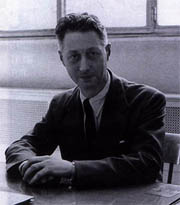
\includegraphics[width=4cm]{Bezier.jpg}
	\caption{Pierre B\'{e}zier, 1958}
\end{figure}

\indent 
Math\'{e}maticien, physicien, philosophe, ing\'{e}nieur en m\'{e}canique et en \'{e}lectricit\'{e}, il est renomm\'{e} pour ses inventions r\'{e}volutionnaires pour lesquelles il re\c coit le Prix Nessim-Habif en 1972. \`{a} l'\'{e}poque, un \'{e}l\'{e}ment nouveau vient tout remettre en cause : le d\'{e}veloppement des machines \`{a} commande num\'{e}rique. Apparues chez Renault au d\'{e}but des ann\'{e}es soixante, elles n'\'{e}taient programm\'{e}es que de fa\c con relativement simple. Pierre B\'{e}zier chercha donc comment traduire math\'{e}matiquement une courbe, puis une surface dessin\'{e}e \`{a} main lev\'{e}e, ce qui rend plus facile pour la commande num\'{e}rique de prendre en compte instinctivement les modifications apport\'{e}es \`{a} un mod\`{e}le. Il s'attaque alors au probl\`{e}me de la mod\'{e}lisation des surfaces en trois dimensions, les commandes num\'{e}riques se contentant jusqu'alors de courbes en deux dimensions. Comme B\'{e}zier voulait une interface accessible \`{a} toute le monde, il d\'{e}cide alors de consid\'{e}rer classiquement les surfaces comme une transformation de courbes. Son exigence de s'adapter au dessinateur l'am\`{e}ne \`{a} une invention g\'{e}niale, \`{a} savoir d\'{e}duire le calcul \`{a} partir du dessin gr\^{a}ce \`{a} sa propre technique innovatrice nomm\'{e}e \guillemotleft $\;$poign\'{e}e de contr\^{o}le \guillemotright.

\begin{figure}[h]
	\centering
	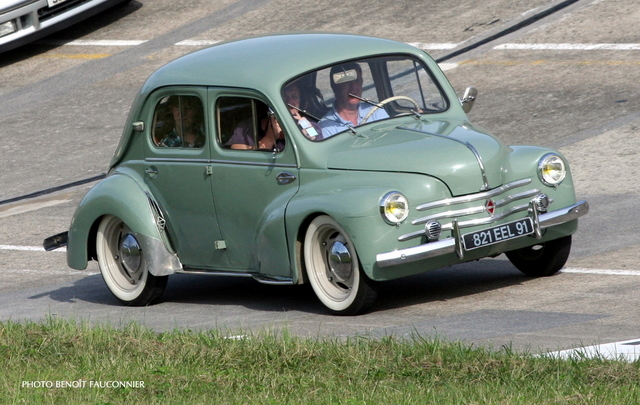
\includegraphics[width=6cm]{renault_4.jpg}
	\caption{Renault 4CV}
\end{figure}

\indent	
	Au lancement de la Renault 4CV, en 1946, son objectif, tr\`{e}s ambitieux pour l'\'{e}poque, est d'assurer une cadence de 20 voitures par jour. Pour cela, il imagine une machine transfert \`{a} t\^{e}tes ind\'{e}pendantes. En un an, son \'{e}quipe r\'{e}alise 750 unit\'{e}s d'usinage normalis\'{e}es et 60 tables rotatives. Ainsi, la cadence atteint progressivement 300 voitures par jour. Ces machines sp\'{e}ciales sont vendues \`{a} travers le monde. Il devient alors chef du bureau d'\'{e}tudes outillages m\'{e}caniques. En 1955, il s'int\'{e}resse \`{a} la commande num\'{e}rique et trois ans plus tard, il met au point des perceuses avec des \'{e}quipements aux commandes enti\`{e}rement transistoris\'{e}es. Il avance successivement sur l'\'{e}chelle hi\'{e}rarchique jusqu'en 1960 o\`{u} il est nomm\'{e} directeur g\'{e}n\'{e}rale, d\'{e}charg\'{e} de toute responsabilit\'{e} op\'{e}rationnelle.
\par
B\'{e}zier \'{e}tait un ing\'{e}nieur tr\`{e}s rigoureux qui avait une affinit\'{e} formidable pour la pr\'{e}cision des r\'{e}sultats en visualisant la mod\'{e}lisation comme une \oe{}uvre d'art. Par cons\'{e}quent, il choisit la voie la plus difficile \`{a} explorer, \`{a} savoir transformer les courbes de forme des stylistes de carrosserie en expressions math\'{e}matiques qui devaient \^{e}tre utilisables par les ing\'{e}nieurs gr\^{a}ce aux ordinateurs et ses liaisons avec les machines-outils. Ses recherches aboutirent \`{a} un logiciel appel\'{e} Unisurf. 
\\\\
\textbf{Unisurf}\\
Unisurf (\guillemotleft $\;$uni \guillemotright $\;$pour unification et \guillemotleft $\;$surf \guillemotright $\;$pour surface) est un pionnier des logiciels de DAO (Dessin Assist\'{e} par Ordinateur) et de CFAO (Conception et Fabrication Assist\'{e}es par Ordinateur). Unisurf a \'{e}t\'{e} d\'{e}velopp\'{e} en 1971 par Pierre B\'{e}zier ayant pour but de passer directement du papier \`{a} la machine. Cette application, destin\'{e}e \`{a} la conception des automobiles en association directe avec les machines \`{a} commandes num\'{e}riques est la base des logiciels de CFAO (par exemple CATIA) d\'{e}velopp\'{e}s ult\'{e}rieurement. Unisurf provoque au d\'{e}but un mini tsunami culturel. En fait, les premi\`{e}res pi\`{e}ces qui pouvaient \^{e}tre r\'{e}alis\'{e}es gr\^{a}ce \`{a} la CAO \'{e}taient des pi\`{e}ces petites peu compliqu\'{e}es et les dessinateurs regardaient ce logiciel avec scepticisme car dessiner avec le logiciel prenait plus de temps que de le r\'{e}aliser sur papier. De plus, les logiciels et les machines provoquaient souvent des erreurs \`{a} cause de mauvaises manipulations et des petits moteurs des tables \`{a} dessin qui se bloquaient. Toutefois, l'\'{e}volution a \'{e}t\'{e} extraordinaire et peu \`{a} peu Renault passe de 10\% des pi\`{e}ces fabriqu\'{e}es par CAO \`{a} 30\% puis \`{a} 60\%.
\\
\indent	
En 1968, Unisurf est pr\'{e}sent partout, en particulier \`{a} D\'{e}troit, le temple de l'industrie automobile \`{a} l'\'{e}poque. Une machine \`{a} dessiner, une fraiseuse, un ordinateur d'occasion avec une m\'{e}moire de 8 ko et un logiciel rudimentaire. Le syst\`{e}me est op\'{e}rationnel en 1972 et avec Unisurf 3 en 1975, la CFAO se g\'{e}n\'{e}ralise dans toute l'industrie, facilitant la d\'{e}finition graphique d'objets aux formes complexes (nez des motrices TGV, si\`{e}ges de voiture etc.).
\par
Cette mod\'{e}lisation math\'{e}matique s'appuie sur les fameuses \guillemotleft $\;$courbes de B\'{e}zier \guillemotright, repr\'{e}sentatives de polyn\^{o}mes param\'{e}triques en langage math\'{e}matique. Elles constituent le sujet de sa th\`{e}se de doctorat d'\'{e}tat en math\'{e}matiques d\'{e}fendue le 23 f\'{e}vrier 1977 sous le titre: \guillemotleft $\;$Essai de d\'{e}finition num\'{e}rique des courbes et surfaces \guillemotright.
\\
\indent	
Unisurf est adopt\'{e} en 1967 par Peugeot qui le perfectionne et l'utilise pour concevoir la maquette compl\`{e}te de la Peugeot 104. Peugeot et Renault collaboreront ainsi pendant quinze ans aux versions successives du syst\`{e}me Unisurf. \`{a} partir de 1980, une vingtaine de personnes dont quatre \`{a} cinq informaticiens travaillent chez Renault avec le logiciel Unisurf sur des machines qui occupent l'espace d'une chambre.


\newpage
\subsection{Formulation du probl\`{e}me}
\begingroup\raggedleft
\underline{La probl\'{e}matique}
\endgroup
\par
On consid\`{e}re $n+1$ points du plan ($n \ge 1$, le plus souvent $n = 3$), $A_0 , A_1 , . . ., A_n$ et on d\'{e}finit une courbe param\'{e}tr\'{e}e $M(t)$, $t \in [0, 1]$, associ\'{e}e \`{a} ces points, o\`{u} $M(t)$ est un barycentre des $A_i$ :
\[M(t) = B_0 (t)A_0 + B_1 (t)A_1 + · · · + B_n (t)A_n\]
o\`{u} $M(t)$ $B_i(t) \ge 0 \quad \forall i = 0, ..., n$
\\[2pt]
$\sum B_i (t) = 1 \quad \forall i = 0, ..., n$
\\[10pt]
Les coefficients $B_i(t)$ d\'{e}pendent de t de mani\`{e}re la plus r\'{e}guli\`{e}re possible.
La solution adopt\'{e}e par P. B\'{e}zier consiste \`{a} prendre les polyn\^{o}mes de Bernstein.

\begingroup\raggedleft
\underline{D\'{e}finition}
\endgroup
\\
Les polyn\^{o}mes de Bernstein d'ordre n sont les polyn\^{o}mes \[B_{i, n} (t) = \dbinom{n}{i}t^i(1-t)^{n-i}\]
Lorsque $n$ est fix\'{e}, on note simplement $B_i$ au lieu de $B_{i, n}$. 
\\
On v\'{e}rifie aussit\^{o}t que les $B_i$ sont sup\'{e}rieur \`{a} 0 sur $[0, 1]$ et que leur somme est bien égale \`{a} 1 (c'est la formule du bin\^{o}me de Newton appliqu\'{e}e \`{a} $(1 -t + t)^n$).

\begingroup\raggedleft
\underline{Remarques}
\endgroup
\\[5pt]
1) On a $B_{0, n} (t) = (1-t)^n$ et $B_{n, n} (t) = t^n$
\\
2) On notera que :
\\
- les polyn\^{o}mes $B_i (t)$ forment une base de l'espace vectoriel des polyn\^{o}mes de degr\'{e} inf\'{e}rieur \`{a} $n$ (tous les polyn\^{o}mes sont \'{e}l\'{e}ments de $R^n$)
\\
- l'espace est non nul et stable par combinaison lin\'{e}aire, donc sous-espace vectoriel de $R^n$
\\
3) Les polyn\^{o}mes $B_i$ forment ce qu'on appelle une partition de l'unit\'{e}. Ils sont bien connus en analyse. En particulier, si $f$ est une fonction continue sur $[0, 1]$, on peut poser :
\[B_n (f) = \sum \limits_{\underset{}{i=0}}^n (\frac{i}{n})B_i(f)\]
On montre que la suite de polyn\^{o}mes $B_n (f)$ converge uniform\'{e}ment vers $f$ sur $[0, 1]$ (cela est le th\'{e}or\`{e}me de Weierstrass).

\newpage
\subsection{Partie Math\'{e}matique}

\begingroup\raggedleft
\underline{Th\'{e}orie g\'{e}n\'{e}rale}
\endgroup
\par
Quatre points $P_0 , P_1 , P_2 et P_3$ d\'{e}finissent une courbe de B\'{e}zier cubique. La courbe se trace en partant du point $P_0$, en se dirigeant vers $P_1$ et en arrivant au point $P_3$ selon la direction $P_2-P_3$, mais elle ne passe ni par $P_1$ ni par $P_2$ (ces points donnent une information de direction). La distance entre $P_0$ et $P_1$ d\'{e}termine la "longueur" du d\'{e}placement dans la direction de $P_1$ avant de tourner vers $P_3$.
\\
\indent
    Pour la forme param\'{e}trique de la courbe, nous remarquons que la formule des coefficients du polyn\^{o}me qui caract\'{e}rise la courbe est inspirée d'une loi binomiale et montre que la courbe est toujours totalement contenue dans l'enveloppe convexe des quatre points donn\'{e}s (ce qui aide \'{e}galement \`{a} v\'{e}rifier les conditions de polyn\'{o}mes de Bernstein).
\\
\indent
    Les courbes de B\'{e}zier sont int\'{e}ressantes pour le traitement des images car les points peuvent \^{e}tre rapidement calcul\'{e}s en utilisant une proc\'{e}dure r\'{e}cursive qui utilise la division et les op\'{e}rations de base en \'{e}vitant toutes les opérations de l'arithm\'{e}tique des nombres r\'{e}els flottants.


\[\begin{pmatrix}
A' \\
B' \\
C' \\ 
D'\\
\end{pmatrix}
=
\begin{pmatrix}
1 & 0 & 0 & 0 \\[5pt]
\frac{1}{2} & \frac{1}{2} & 0 & 0 \\[5pt]
\frac{1}{4} & \frac{2}{4} & \frac{1}{4} & 0 \\[5pt]
\frac{1}{8} & \frac{3}{8} & \frac{3}{8} & \frac{1}{8} \\[5pt]
\end{pmatrix}
\begin{pmatrix}
A \\
B \\
C \\ 
D \\
\end{pmatrix}\]
\\
\centerline{ou}
\begin{align*}
& D \leftarrow \frac{C+D}{2}
\\[5pt]
& C \leftarrow \frac{B+C}{2}, \; D \leftarrow \frac{C+D}{2}
\\[5pt]
& B \leftarrow \frac{A+B}{2}, \; C \leftarrow \frac{B+C}{2}, \; D \leftarrow \frac{C+D}{2}
\end{align*}

Plus pr\'{e}cis\'{e}ment, on peut d\'{e}composer la courbe $P(t)$ en deux courbes $P_L$ et $P_R$ dont les points de
contr\^{o}les sont respectivement ($L_1 , L_2 , L_3 , L_4$) et ($R_1 , R_2 , R_3 , R_4$):

\[\begin{pmatrix}
L_1' \\
L_2' \\
L_3' \\ 
L_4'\\
\end{pmatrix}
=
\begin{pmatrix}
1 & 0 & 0 & 0 \\[5pt]
\frac{1}{2} & \frac{1}{2} & 0 & 0 \\[5pt]
\frac{1}{4} & \frac{2}{4} & \frac{1}{4} & 0 \\[5pt] 
\frac{1}{8} & \frac{3}{8} & \frac{3}{8} & \frac{1}{8} \\[5pt]
\end{pmatrix}
\begin{pmatrix}
A \\
B \\
C \\ 
D \\
\end{pmatrix}
\;\;\;\;
et
\;\;\;\;
\begin{pmatrix}
R_1' \\
R_2' \\
R_3' \\ 
R_4'\\
\end{pmatrix}
=
\begin{pmatrix}
\frac{1}{8} & \frac{3}{8} & \frac{3}{8} & \frac{1}{8} \\[5pt]
0 & \frac{1}{4} & \frac{2}{4} & \frac{1}{4} \\[5pt]
0 & 0 & \frac{1}{2} & \frac{1}{2} \\[5pt] 
0 & 0 & 0 & 1 \\[5pt]
\end{pmatrix}
\begin{pmatrix}
A \\
B \\
C \\ 
D \\
\end{pmatrix}\]

\newpage
\begingroup\raggedleft
\underline{Courbes de B\'{e}zier d'ordre 2 (quadratique)}
\endgroup
\par
Une courbe de B\'{e}zier quadratique est la courbe $B(t)$ d\'{e}finie par les points de contr\^{o}le $P_0, P_1$ et $P_2.$
\[B(t) = (1-t)^2 P_0 + 2t (1-t) P_1 + t^2 P_2 , \qquad t \in [0,1]\]
On consid\`{e}re trois points distincts $A, \; B, \; C$ du plan. 
\\
On pose $A = (a_1 , a_2 ), B = (b_1 , b_2 ), C = (c_1 , c_2 )$.
\\
On consid\`{e}re la courbe de B\'{e}zier $\Gamma$ d\'{e}finie par \[M(t) = (1-t)^2 A+ 2t(1-t)B + t^2C\]
Elle passe par $A$ et $C$ et elle est tangente respectivement \`{a} ($AB$) et ($BC$) en ces points. Si $A, B, C$ sont align\'{e}s, la courbe $\Gamma$ est \'{e}gale au segment [$AB$]. Sinon, la courbe $\Gamma$ est une parabole.
\\[10pt]
\underline{D\'{e}monstration pour $A, B, C$ non colin\'{e}aires}:
On a les formules:
\[x(t) = at^2 + bt + c \qquad et \qquad y(t) = a' t^2 + b't + c'\]
avec $a = a_1-2b_1 + c_1, \;\;  b = 2(b_1-a_1 ), \;\; a'’ = a_2-2b_2 + c_2, \;\; b' = 2(b_2-a_2 )$
\par
On note que $a \ne 0$ et $a’ \ne 0$ car sinon $B$ est le milieu de $[AC]$. 
On \'{e}limine les termes en $t^2$ entre ces \'{e}quations: 
\[a’x-ay = (a'b-ab')t + a'c-ac'\]
\indent
Si le coefficient de $t$ est nul on obtient une droite, ce qui est absurde puisque les points $A, B, C$ ne sont pas align\'{e}s (en outre les droites ($AB$) et ($BC$) sont tangentes \`{a} la courbe). Pr\'{e}cis\'{e}ment, ce coefficient vaut \[a’b-ab’ = 2(-a_1 b_2 + b_1 a_2 + c_1 b_2-b_1 c_2 + a_1 c_2-c_1 a_2 )\] 
et c'est le d\'{e}terminant obtenu en bordant d'une ligne de 1 la matrice des coordonn\'{e}es de $A, B, C$.
\\
On peut \'{e}crire une expression pour $t$ comme on est s\^{u}r de ne pas diviser par 0:
\[t = \frac{a'x-ay + ac'-a'c}{a'b-ab'}\]
\indent
Si on d\'{e}signe par $X$ cette quantit\'{e} (ce qui revient \`{a} faire un changement de coordonn\'{e}es
cart\'{e}siennes) l'\'{e}quation de $\Gamma$ s'\'{e}crit $y = a'X 2 + b'X + c'$, ce qui correspond \`{a} l'\'{e}quation d'une parabole.
\\
\indent
Ces courbes quadratiques sont encore tr\`{e}s utilis\'{e}es aujourd'hui (par exemple dans les d\'{e}finitions de glyphes des polices de caract\`{e}res des logiciels de traitement de texte au format TrueType et les polices OpenType dans leur vari\'{e}t\'{e} compatible TrueType).

\newpage
Ce type de courbes permet d'assurer la continuit\'{e} en tangence de deux courbes raccord\'{e}es mais en g\'{e}n\'{e}ral, elles ne permettent pas de conserver la continuit\'{e} de la courbure aux points d'interconnexion. Pour diminuer cet inconv\'{e}nient, il est alors n\'{e}cessaire d'augmenter le nombre d'arcs interconnect\'{e}s afin de r\'{e}duire les ruptures de courbure entre chacun d'eux, ce qui en limite l'int\'{e}r\^{e}t et peut conduire \`{a} une complexification de la conception des courbes (avec davantage de sommets et de points de contr\^{o}les \`{a} positionner).
\\[10pt]
\underline{Courbes de B\'{e}zier d'ordre 3 (cubiques)}
\par
Une courbe de B\'{e}zier cubique est la courbe $B(t)$ d\'{e}finie par les points de contr\^{o}le $P_0 , P_1 , P_2 \;\; et \;\; P_3$.
Sa forme param\'{e}trique est:
\[B(t) = P_0 (1-t)^3 + 3P_1 t(1-t)^2 + 3P_2 t ^2 (1-t) + P_3 t^3 , \qquad t \in [0,1]\]
\indent  
Ce sont les courbes de B\'{e}zier qui sont les plus utilis\'{e}es en conception graphique car elles permettent d'assurer non seulement la continuit\'{e} en tangence de deux courbes raccordées mais aussi celle de leur courbure en \'{e}vitant de positionner de nombreux sommets et points de contr\^{o}le comme en ordre 2. Elles sont utilis\'{e}es pour les polices des logiciels de traitement de texte par exemple dans le langage PostScript et la d\'{e}finition des glyphes des polices de caract\`{e}res de \guillemotleft $\;$type 1 \guillemotright, ainsi que dans les polices OpenType dans leur vari\'{e}t\'{e} CFF (Compact Font Format) qui reprennent les m\^{e}mes d\'{e}finitions de sommets et de points de contr\^{o}le.
\par
Il en r\'{e}sulte un th\'{e}or\`{e}me g\'{e}n\'{e}ral prouv\'{e} ci-dessous que la courbe est une portion cubique, c'est-\`{a}-dire qu'elle est d\'{e}finie par une \'{e}quation $F(x, y) = 0$ o\`{u} $F$ est un polyn\^{o}me de degr\'{e} inf\'{e}rieur ou \'{e}gal \`{a} 3. Les polyn\^{o}mes de Bernstein $(1-t)^3, \;\; 3(1-t)^2 t, \;\; 3(1-t)t^2$ et $t^3$ constituent une base de l'espace vectoriel des polyn\^{o}mes de degr\'{e} inf\'{e}rieur ou \'{e}gal \`{a} 3.
\\[10pt]
\underline{D\'{e}monstration} : on a quatre points $A, \; B, \; C, \; D$ et on pose :
\[M(t) = (1 − t)^3 A + 3(1 − t)^2 t B + 3(1 − t)t^2 C + t^3 D\]
\indent
Il suffit de noter que leurs valeurs sont respectivement 0, 1, 2, 3. Par cons\'{e}quent, les courbes de B\'{e}zier d'ordre 3 sont exactement toutes les courbes param\'{e}tr\'{e}es par des polyn\^{o}mes de degr\'{e} inf\'{e}rieur ou \'{e}gal \`{a} 3. En effet, si on pose $A = (a_1, a_2), \; B = (b_1 , b_2 )$ et de m\^{e}me pour tous les points, on obtient tous les couples de polyn\^{o}mes de degré inf\'{e}rieur ou \'{e}gal \`{a} 3 possibles. Les courbes de B\'{e}zier sont des courbes de degré 3. Elles sont donc d\'{e}termin\'{e}es par quatre points de contr\^{o}le. Si les coordonn\'{e}es des points de contr\^{o}le sont $(x_1, y_1), \; (x_2, y_2), \; (x_3, y_3)$ et $(x_4, y_4)$,
l'\'{e}quation de la courbe est :
\\[5pt]
$x(t) = (1-t)^3 x_1 + 3t(1-t)^2 x_2 + 3t^2 (1-t)x_3 + t^3 x_4$ pour $0 \leq t \leq 1$
\\[5pt]
$y(t) = (1-t)^3 y_1 + 3t(1-t)^2 y_2 + 3t^2 (1-t)y_3 + t^3 y_4$ pour $0 \leq t \leq 1$

\newpage
\section{Splines cubiques} 
\subsection{Contexte} 

Quand on parle de l'interpolation math\'{e}matiques, on s'int\'{e}resse aux m\'{e}thodes de mod\'{e}lisation et param\'{e}trisation des courbes entre plusieurs points de contr\^{o}le d\'{e}j\`{a} fix\'{e}s \`{a} l'aide des fonctions fondamentales. Les polyn\^{o}mes sont tr\`{e}s bien adapt\'{e}s pour ce genre de probl\`{e}mes gr\^{a}ce \`{a} leurs particularit\'{e}s qui favorisent une r\'{e}solution simple et rapide. 
\\
\indent
Cependant, comme leur pr\'{e}cision n'est pas tr\`{e}s \'{e}lev\'{e}e, dans les probl\`{e}mes d'interpolation on pr\'{e}f\`{e}re utiliser les splines dans la majorit\'{e} des cas puisque on trouve des r\'{e}sultats similaires avec les interpolations polynomiales de degr\'{e} tr\`{e}s grand tout en \'{e}vitant les instabilit\'{e}s dus au Ph\'{e}nom\`{e}ne du Runge que peuvent entra\^{i}ner des r\'{e}sultats avec une pr\'{e}cision moyenne. En effet, au niveau des graphiques num\'{e}riques, les splines cubiques sont les fondements des nombreuses op\'{e}rations gr\^{a}ce \`{a} la simplicit\'{e} de construction, \`{a} la pr\'{e}cision assez importante des solutions et \'{e}galement \`{a} leur capacit\'{e} de d\'{e}crire des formes complexes avec des ajustements et design interactif des courbes. 
L'\'{e}volution des splines est notamment observ\'{e}e apr\`{e}s l'apparition des ordinateurs. En s'appuyant sur l'interpolation polynomiale d\'{e}j\`{a} pr\'{e}sente \`{a} l'\'{e}poque, les scientifiques et les math\'{e}maticiens ont d\'{e}velopp\'{e} une m\'{e}thode d'interpolation par morceaux de polyn\^{o}mes afin d'augmenter l'efficacit\'{e} des r\'{e}sultats tout en gardant la m\^{e}me simplicit\'{e} de manipulation. 
\\
\indent
Un des plus importants fondateurs des m\'{e}thodes de l'interpolation en utilisant des polyn\^{o}mes d\'{e}finis par morceaux est Isaac Schoenberg. Math\'{e}maticien roumain n\'{e} au d\'{e}but du XX\`{e}me si\`{e}cle, r\'{e}put\'{e} pour ses travaux sur les splines, fait ses \'{e}tudes notamment en Roumanie, Allemagne et \'{e}galement aux \'{e}tats-Unis. Vers 1940, Schoenberg a r\'{e}alis\'{e} des travaux extr\^{e}mement importants sur le sujet de l'analyse math\'{e}matiques g\'{e}n\'{e}rale et sur le sujet d'approximation en utilisant l'interpolation par des fonctions splines d\'{e}velopp\'{e}es par lui m\^{e}me. Pendant 15 ann\'{e}es, il est le seul qui s'int\'{e}resse \`{a} ce type d'interpolation en r\'{e}ussissant \`{a} \'{e}crire une quarantaine de documents qui seront indispensables pour les ouvrages d\'{e}velopp\'{e}s plus tard par d'autres scientifiques. De ce fait, en 1960, quand les ordinateurs sont de plus en plus r\'{e}pandus dans le monde scientifique, on commence \`{a} utiliser les splines notamment pour les ajustements des donn\'{e}es num\'{e}riques et pour le design g\'{e}om\'{e}trique assist\'{e} par ordinateur (ce qui est \`{a} la base de la CAO moderne qui actuellement utilise les B-splines, plus \'{e}volu\'{e}s). Malgr\'{e} sa retraite prise en 1973, il n'arr\^{e}te pas ses  recherches sur les splines, ce qui lui permet d'introduire un autre concept d'importance majeure, \`{a} savoir les splines cardinales.
\\
\indent
	Une courbe spline est une fonction polynomiale par morceaux d\'{e}finie sur un intervalle [a;b] divis\'{e} en sous-intervalles. Le degr\'{e} de la spline est d\'{e}fini comme celui du polyn\^{o}me de plus haut degr\'{e} utilis\'{e} dans sa construction. On appelle spline uniforme, une spline construite sur l'intervalle [a;b] seulement avec des polyn\^{o}mes qui ont le m\^{e}me degr\'{e}. Dans le cas contraire, elle est non uniforme.
	\\
\indent
En ce qui concerne la d\'{e}rivabilit\'{e} d'une spline, sachant que la d\'{e}rivabilit\'{e} d'un polyn\^{o}me est infinie, elle d\'{e}pend de la continuit\'{e} au niveau de la jointure des courbes polynomiales d\'{e}finies sur chaque sous-intervalle de [a;b].
\\
\indent
La plus simple fonction spline est celle uniforme de degr\'{e} 1 appel\'{e} aussi ligne polygonale ou ligne bris\'{e}e. Graphiquement, la m\'{e}thode consiste juste \`{a} relier chaque point avec des segments de droite, ce qui donnera une continuit\'{e} $C^0$ sauf si les points sont align\'{e}s.
\\
\indent
	Le cas le plus courant et le plus important des splines est la spline cubique uniforme. Ces fonctions ont une utilit\'{e} fondamentale dans une large gamme de domaines scientifiques, notamment dans la CAO. En fonction des contraintes impos\'{e}es en g\'{e}n\'{e}ral par la sp\'{e}cificit\'{e} de chaque probl\`{e}me, on a multiples mani\`{e}res d'interpoler:
\begin{itemize}
\item [$\bullet$] Interpolation avec les tangentes
\item [$\bullet$] Interpolation avec m\'{e}thode de Catmull-Rom
\begin{itemize}
\item[o] Spline circulaire
\item[o]Spline serr\'{e}e
\item[o] Spline naturelle
\end{itemize}
\item [$\bullet$] Interpolation en courbure
\end{itemize}

\newpage
\subsection{R\'esolution math\'ematique} 
\begingroup\raggedleft
\underline{D\'{e}finition}
\endgroup

Consid\'{e}rons $n+1$ points $x_i$ distincts. On d\'{e}finit un polyn\^{o}me $s_i$ sur \\
$I = [x_i, \; x_{i+1}]$ tel que \[s_i(x) = a_ix³ + b_ix² + c_ix + d_i\qquad avec \;\;\; i= 0, 1, 2,..., n\]

Posons
\[s_i(x_i)= f(x_i) = f_i\]

On doit avoir $s$ $\in C^2$. Nous devons donc satisfaire le syst\`{e}me suivant: \par
$\begin{cases}
s'_{i-1}(x_i)=s'_i(x_i)\;\;\;\;\;\;\;\;\;\;\;\;\;\;i=1,2,...,{n-1}\\
s''_{i-1}(x_i)=s''_i(x_i)
\end{cases}$
\\
\par
On obtient 
\begin{center}
\fbox{$s''_i(x) = f''_i \frac{(x_{i+1}-x)}{h_i} + f''_{i+1} \frac{(x-x_i)}{h_i}$} \;\;\;\;\;\; o\`u \; $h_i=x_{i+1}-x_i$
\end{center}

\underline{D\'{e}monstration}
\[s_i(x_i) = a_ix_i^{3} + b_ix_i^{2} + c_ix_i + d_i\]
\par
\begingroup\raggedleft
En d\'{e}rivant:
\endgroup 
\begin{align*} 
s'_i(x_i) & = 3a_ix_i^{2} + 2b_ix_i + c_i
\\[5pt] 
s''_i(x_i) & = 6a_ix_i + 2b_i
\end{align*} 
\\
\[\Rightarrow b_i=\frac{s''_i(x_i)-6a_ix_i}{2}=\frac{f''_i-6a_ix_i}{2}\] 

\begingroup\raggedleft
De plus,
\endgroup  
\begin{align*} 
s''_i&(x_{i+1})= 6a_i(x_{i+1})+2b_i 
\\[5pt]
b_i&=6a_ix_{i+1}+2\frac{(s''_i(x_i)-6a_ix_i)}{2}
\\[15pt]
s''_i&(x_{i+1})= 6a_ix_{i+1}+f''_i-6a_ix_i= f''_{i+1}
\\[5pt]
a_i&[6(x_{i+1})-6x_i]=f''_{i+1}-f''_i
\\[5pt]
a_i & =\frac{(f''_{i+1}-f''_i)}{6(x_{i+1}-x_i)} 
\end{align*} 
\\
On a \[s''_i(x) = 6a_ix + 2b_i\]
\\
En rempla\c cant $a_i$ et $b_i$ par leurs expressions, on obtient : 
\begin{align*} 
s''_i(x)&=6\frac{(f''_{i+1}-f''_i)}{6(x_{i+1}-x_i)}x + 2\frac{(f''_i-6a_ix_i)}{2}
\\[5pt]
s''_i(x)&=\frac{(f''_{i+1}-f''_i)}{x_{i+1}-x_i}x + f''_i-6a_ix_i
\\[5pt]
s''_i(x)&=\frac{(f''_{i+1}-f''_i)}{x_{i+1}-x_i}x + f''_i-6\frac{(f''_{i+1}-f''_i)}{6(x_{i+1}-x_i)}x_i
\\[5pt]
s''_i(x)&= \frac{x(f''_{i+1}-f''_i)}{(x_{i+1}-x_i)} + f''_i-\frac{x_i(f''_{i+1}-f''_i)}{(x_{i+1}-x_i)}
\end{align*} 
\\
Or $h_i=x_{i+1}-x_i$,
\begin{align*} 
s''_i(x) & = \frac{x(f''_{i+1}-f''_i)}{(x_{i+1}-x_i)} + f''_i-\frac{x_i(f''_{i+1}-f''_i)}{(x_{i+1}-x_i)}
\\[5pt]
s''_i(x) & = \frac{xf''_{i+1}-xf''_i + f''_i(x_{i+1}-x_i)-x_if''_{i+1}+ x_if''_i}{h_i}
\\[5pt]
s''_i(x) & = \frac{xf''_{i+1}-xf''_i + x_{i+1}f''_i-x_if''_i-x_if''_{i+1}+ x_if''_i}{h_i}
\\[5pt]
s''_i(x) & = \frac{f''_{i+1}(x-x_i) + f''_i(x_{i+1}-x)}{h_i}
\\[5pt]
s''_i(x)&= f''_i\frac{(x_{i+1}-x)}{h_i} + f''_{i+1}\frac{(x-x_i)}{h_i}
\end{align*} 

\begingroup\raggedleft
On int\`{e}gre deux fois et en consid\'{e}rant les constantes d'int\'{e}gration $a_i$ et $b_i$ :
On int\`{e}gre une premi\`{e}re fois :
\endgroup
\begin{align*} 
s'_i(x)&=\int\! (f''_i\frac{(x_{i+1}-x)}{h_i} + f''_{i+1}\frac{(x-x_i)}{h_i}) \, \mathrm{d}x
\\[5pt]
s'_i(x)&= -f''_i\frac{(x_{i+1}-x)^2}{2h_i} + a_i +  f''_{i+1}\frac{(x-x_i)^2}{2h_i} + b_i
\end{align*} 
\\
On int\'{e}gre une deuxi\'{e}me fois :
\\
\begin{align*} 
s_i(x)&=\int\! (-f''_i\frac{(x_{i+1}-x)^2}{2h_i} + a_i +  f''_{i+1}\frac{(x-x_i)^2}{2h_i} + b_i) \, \mathrm{d}x
\\[5pt]
s_i(x)& = f''_i \frac{(x_{i+1}-x)^3}{6h_i}+ f''_{i+1} \frac{(x-x_i)^3}{6h_i}+a_i(x_{i+1}-x) + b_i (x-x_i) \qquad i= 0,1,...,n-1 
\end{align*} 
\\
Nous allons maintenant d\'{e}terminer les expressions de $a_i$ et $b_i$ :

\begingroup\raggedleft
Ces constantes peuvent \^{e}tre d\'{e}termin\'{e}es en \'ecrivant les relations de continuit\'{e} aux noeuds.
\endgroup
\[s_i(x_i) = f(x_i) \;\; et \;\; s_i(x_{i+1})=f(x_{i+1})\]
Pour $a_i$ :
\begin{align*} 
s_i&(x_i) = f''_i \frac{(x_{i+1}-x_i)^3}{6h_i}+ f''_{i+1} \frac{(x_i-x_i)^3}{6h_i}+a_i(x_{i+1}-x_i) + b_i (x_i-x_i) \;\; avec \;\; h_i=x_{i+1}-x_i
\\[5pt]
f_i& = f''_i \frac{h_i^2}{6}+a_ih_i
\\[5pt]
a_i& = \frac{{(f_i-f''_i)}\frac{h_i^2}{6}}{h_i}
\\[5pt]
a_i&= \frac{f_i}{h_i}-f''_i \frac{h_i}{6}
\end{align*} 

\begin{align*} 
\textrm{Pour} & \; b_i :
\\[5pt]
s_i(x&_{i+1}) = f''_i \frac{(x_{i+1}-x_{i+1})^3}{6h_i}+ f''_{i+1} \frac{(x_{i+1}-x_i)^3}{6h_i}+a_i(x_{i+1}-x_{i+1}) + b_i (x_{i+1}-x_i) \;\; avec \;\; h_i=x_{i+1}-x_i
\\[5pt]
f_{i+1}& = f''_{i+1} \frac{h_i^2}{6} + b_ih_i
\\[5pt]
b_i = &\frac{{(f_{i+1}-f''_{i+1})}\frac{h_i^2}{6}}{h_i}
\\[5pt]
b_i= &\frac{f_{i+1}}{h_i}-f''_{i+1} \frac{h_i}{6}
\\[10pt]
\textrm{ainsi} & \qquad a_i= \frac{f_i}{h_i}-f''_i \frac{h_i}{6} \;\; et \;\; b_i= \frac{f_{i+1}}{h_i}-f''_{i+1}\frac{h_i}{6}
\end{align*}

\begingroup\raggedleft
On peut alors remplacer les expressions de $a_i$ et $b_i$ dans $s_i(x)$
\endgroup
\[s_i(x) = f''_i \frac{(x_{i+1}-x)^3}{6h_i}+ f''_{i+1} \frac{(x-x_i)^3}{6h_i}+a_i(x_{i+1}-x) + b_i (x-x_i) \qquad i= 0,1,...,n-1 \]
\[s_i(x) = f''_i \frac{(x_{i+1}-x)^3}{6h_i}+ f''_{i+1} \frac{(x-x_i)^3}{6h_i}+ (\frac{f_i}{h_i}-f''_i\frac{h_i}{6})(x_{i+1}-x) + (\frac{f_{i+1}}{h_i}-f''_{i+1}\frac{h_i}{6})(x-x_i)\]
\[s_i(x) = f''_i(\frac{(x_{i+1}-x)^3}{6h_i}-\frac{h_i}{6}(x_{i+1}-x)) + f''_{i+1}(\frac{(x-x_i)^3}{6h_i}-\frac{h_i}{6}(x-x_i)) + \frac{f_i}{h_i}(x_{i+1}-x) + \frac{f_{i+1}}{h_i}(x-x_i)\]

\begin{flushleft}
	Il faut ensuite respecter les conditions de continuit\'{e} pour les d\'{e}riv\'{e}es premi\`{e}res :
\end{flushleft}
\[s_i'(x) = f''_i(\frac{-(x_{i+1}-x)^2}{2h_i}+\frac{h_i}{6}) + f''_{i+1}(\frac{(x-x_i)^2}{2h_i}-\frac{h_i}{6}) - \frac{f_i}{h_i} + \frac{f_{i+1}}{h_i}\]

\newpage
\begingroup\raggedleft
La condition de continuit\'{e} $s_i'(x_i) = s_{i-1}'(x_i)$ en $x_i$ s'\'{e}crit alors :
\endgroup
\\[8pt]
d'une part,
\begin{align*}
s_i'(x_i) & = f''_i(\frac{-(x_{i+1}-x_i)^2}{2h_i}+\frac{h_i}{6}) + f''_{i+1}(\frac{(x_i-x_i)^2}{2h_i}-\frac{h_i}{6}) - \frac{f_i}{h_i} + \frac{f_{i+1}}{h_i}
\\[5pt]
s_i'(x_i) & = f''_i(-\frac{h_i}{2}+\frac{h_i}{6}) - f''_{i+1}\frac{h_i}{6} - \frac{f_i}{h_i} + \frac{f_{i+1}}{h_i}
\\[5pt]
s_i'(x_i) & = f''_i(-\frac{2h_i}{6}) - f''_{i+1}\frac{h_i}{6} - \frac{f_i}{h_i} + \frac{f_{i+1}}{h_i}
\\[5pt]
s_i'(x_i) & = -f''_i\frac{h_i}{3} - f''_{i+1}\frac{h_i}{6} - \frac{f_i}{h_i} + \frac{f_{i+1}}{h_i}
\end{align*}
d'autre part,
\begin{align*}
s_{i-1}'(x_i)& = f''_{i-1}(\frac{-(x_i-x_i)^2}{2h_{i-1}}+\frac{h_{i-1}}{6}) + f''_i(\frac{(x_i-x_{i-1})^2}{2h_{i-1}}-\frac{h_{i-1}}{6}) - \frac{f_{i-1}}{h_{i-1}} + \frac{f_{i}}{h_{i-1}}
\\[5pt]
s_{i-1}'(x_i)& = f''_{i-1}\frac{h_{i-1}}{6} + f''_i(\frac{h_{i-1}^2}{2h_{i-1}}-\frac{h_{i-1}}{6}) - \frac{f_{i-1}}{h_{i-1}} + \frac{f_{i}}{h_{i-1}} \;\ avec \;\; h_{i-1}=x_i-x_{i-1}
\\[5pt]
s_{i-1}'(x_i)& = f''_{i-1}\frac{h_{i-1}}{6} + f''_i(\frac{h_{i-1}}{2}-\frac{h_{i-1}}{6}) - \frac{f_{i-1}}{h_{i-1}} + \frac{f_{i}}{h_{i-1}}
\\[5pt]
s_{i-1}'(x_i)& = f''_{i-1}\frac{h_{i-1}}{6} + f''_i\frac{h_{i-1}}{3} - \frac{f_{i-1}}{h_{i-1}} + \frac{f_{i}}{h_{i-1}}
\end{align*}
\\
ainsi, en utilisant le raccord des d\'{e}riv\'{e}es premi\`{e}res, on a :
\begin{align*}
&s_i'(x_i) = s_{i-1}'(x_i)
\\[5pt]
&-f''_i\frac{h_i}{3} - f''_{i+1}\frac{h_i}{6} - \frac{f_i}{h_i} + \frac{f_{i+1}}{h_i} = f''_{i-1}\frac{h_{i-1}}{6} + f''_i\frac{h_{i-1}}{3} - \frac{f_{i-1}}{h_{i-1}} + \frac{f_{i}}{h_{i-1}}
\\[5pt]
&- \frac{f_i}{h_i} + \frac{f_{i+1}}{h_i} + \frac{f_{i-1}}{h_{i-1}} - \frac{f_{i}}{h_{i-1}} = f''_i\frac{h_i}{3} + f''_{i+1}\frac{h_i}{6} + f''_{i-1}\frac{h_{i-1}}{6} + f''_i\frac{h_{i-1}}{3}
\\[5pt]
&\frac{f_{i+1}-f_i}{h_i} - \frac{f_{i}-f_{i-1}}{h_{i-1}} =\frac{2f''_ih_i+f''_{i+1}h_i+f''_{i-1}h_{i-1}+2f''_ih_{i-1} }{6} 
\\[5pt]
&6(\frac{f_{i+1}-f_i}{h_i} - \frac{f_{i}-f_{i-1}}{h_{i-1}}) = 2f''_i(h_i+h_{i-1})+f''_{i+1}h_i+f''_{i-1}h_{i-1}
\\[5pt]
&h_i f''_{i+1} +2(h_i+h_{i-1})f''_i + h_{i-1}f''_{i-1}=6(\frac{f_{i+1}-f_i}{h_i}-\frac{f_i-f_{i-1}}{h_{i-1}})  \qquad i= 1,2,...,n-1 
\end{align*}
\begingroup\raggedleft
On obtient donc un syst\`{e}me lin\'{e}aire de (n-1) \'{e}quations \`a (n+1) inconnus. Si on fixe les valeurs de $f''_0$ et $f''_n$ (par exemple \`a 0) on peut r\'{e}soudre ce syst\`{e}me.  
\endgroup

\newpage
\subsection{M\'ethode de calcul}

Dans cette section, nous allons montrer comment r\'{e}soudre ce syt\`{e}me pour des points donn\'{e}es.
Consid\'{e}rons 5 points:  $x_0$, $x_1$, $x_2$, $x_3$, et $x_4$, d'ordonn\'{e}es respectives $f_0$, $f_1$, $f_2$, $f_3$, et $f_4$. En appliquant l'\'{e}galit\'{e} (1), on obtient :

\[\left\{\begin{array}{ll}h_0f''_0+2(h_1+h_0)f''_1+h_1f''_2=6(\frac{f_{2}-f_1}{h_1}-\frac{f_1-f_{0}}{h_{0}})\\
h_1f''_1+2(h_2+h_1)f''_2+h_2f''_3=6(\frac{f_{3}-f_2}{h_2}-\frac{f_2-f_{1}}{h_{1}})\\
h_2f''_2+2(h_3+h_2)f''_3+h_3f''_4=6(\frac{f_{4}-f_3}{h_3}-\frac{f_3-f_{2}}{h_{2}})\\
\end{array}\right. \]

Pour une r\'{e}solution plus facile, on peut r\'{e}\'{e}crire le syst\`{e}me sous forme matricielle en factorisant par $f''_0$, $f''_1$, $f''_2$, $f''_3$, $f''_4$, 
on obtient :
\[\begin{pmatrix}
     h_0 & 2(h_1+h_0) & h_1 & 0 & 0 \\
   0 & h_1 & 2(h_2+h_1) & h_2 & 0 \\
   0 & 0 & h_2 & 2(h_3+h_2) & h_3 
 \end{pmatrix} 
\begin{pmatrix}
   f''_0 \\
   f''_1 \\
   f''_2 \\
   f''_3 \\
   f''_4 \\
\end{pmatrix}
=
\begin{pmatrix}
6(\frac{f_{2}-f_1}{h_1}-\frac{f_1-f_{0}}{h_{0}})\\
6(\frac{f_{3}-f_2}{h_2}-\frac{f_2-f_{1}}{h_{1}})\\
6(\frac{f_{4}-f_3}{h_3}-\frac{f_3-f_{2}}{h_{2}})
\end{pmatrix}\]
\\
On obtient un syst\`{e}me de 3 \'{e}quations \`a 5 inconnues ($f''_0$,$f''_1$,$f''_2$,$f''_3$ et $f''_4$), il faut donc compl\'{e}ter ce syst\`{e}me par 2 autres relations afin de pouvoir le r\'{e}soudre. On va donc imposer les valeurs des d\'{e}riv\'{e}es secondes nulles aux deux extr\'{e}mit\'{e}s, soit $f''(x_0)$ = 0 et $f''(x_5)$ = 0. On qualifie alors la courbe obtenue de spline naturelle. En rajoutant ces deux \'{e}quations dans les matrices, on obtient : 
\[\begin{pmatrix}
   1 & 0 & 0 & 0 & 0 \\
   h_0 & 2(h_1+h_0) & h_1 & 0 & 0 \\
   0 & h_1 & 2(h_2+h_1) & h_2 & 0 \\
   0 & 0 & h_2 & 2(h_3+h_2) & h_3 \\
   0 & 0 & 0 & 0 & 1 \\
\end{pmatrix}
\begin{pmatrix}
   f''_0 \\
   f''_1 \\
   f''_2 \\
   f''_3 \\
   f''_4 \\
\end{pmatrix}
=
\begin{pmatrix}
  0\\
6(\frac{f_{2}-f_1}{h_1}-\frac{f_1-f_{0}}{h_{0}})\\
6(\frac{f_{3}-f_2}{h_2}-\frac{f_2-f_{1}}{h_{1}})\\
6(\frac{f_{4}-f_3}{h_3}-\frac{f_3-f_{2}}{h_{2}})\\
0
\end{pmatrix}\]

\newpage
\begingroup\raggedleft
On g\'{e}n\'{e}ralise alors \`{a} $n+1$ points:
\endgroup
\begin{addmargin}[-5em]{-4em}
\[\underbrace{
	\begin{pmatrix}
   1 & 0 & \ldots& \ldots& \ldots& 0 \\
   h_0 & 2(h_1+h_0) & h_1 & \ddots& \ddots& \vdots \\
	0 & h_1 & 2(h_2+h_1) & h_2 & \ddots & \vdots \\
   \vdots & \ddots & \ddots & \ddots & \ddots& \vdots \\
   \vdots & \ddots & \ddots & \ddots & \ddots& \vdots \\
   \vdots & \ddots & \ddots & \ddots & \ddots& \vdots \\
   \vdots & \ddots &\ddots & h_{n-2} & 2(h_{n-1}+h_{n-2}) 		& h_{n-1}\\
   0 & \ldots& \ldots& \ldots& 0 & 1
 \end{pmatrix}
}_{A}
\underbrace{
\begin{pmatrix}
   f''_0 \\
   f''_1 \\
   f''_2 \\
   f''_3\\
   \vdots\\\
   \vdots\\
    f''_{n-1} \\
    f''_n \\
 \end{pmatrix}
}_{X}
=
\underbrace{
\begin{pmatrix}
  0\\
6(\frac{f_{2}-f_1}{h_1}-\frac{f_1-f_{0}}{h_{0}})\\
6(\frac{f_{3}-f_2}{h_2}-\frac{f_2-f_{1}}{h_{1}})\\
  \vdots\\
   \vdots\\\
   \vdots\\
6(\frac{f_{n}-f_{n-1}}{h_{n-1}}-\frac{f_n-f_{n-2}}{h_{n-2}})\\
0
 \end{pmatrix}
}_{G}\]
\end{addmargin}

\begingroup\raggedleft
On peut remarquer que l'on obtient un syst\`{e}me de la forme AX=G de dimension (n+1). Pour le r\'{e}soudre, nous utilisons l'algorithme de Thomas. 
\endgroup

\paragraph{Algorithme de Thomas:}
La r\'{e}solution du syst\`{e}me AX=G est alors ramen\'{e}e \`{a} la r\'{e}solution successive des syst\`{e}mes UX=Y et LY=G, pour ensuite avoir LUX=G, ce qui \'{e}quivaut \`a AX=G.

\paragraph{Calcul de L et U:}
Soit la matrice A, avec des coefficients simplifi\'{e}s :

\[A=\begin{pmatrix}
   s_1 & w_1 & 0 & \ldots & \ldots & 0 \\
   e_2 & s_2 & w_2 & \ddots & \ddots & \vdots \\
   0 & \ddots & \ddots & \ddots & \ddots & \vdots \\
   \vdots & \ddots & \ddots & \ddots & \ddots & 0 \\
   \vdots & \ddots & \ddots & e_{n-1} & s_{n-1} & w_{n-1} \\
   0 & \ldots & \ldots & 0 & e_n & s_n
\end{pmatrix}\]

\newpage
\begingroup\raggedleft
On cherche des matrices L et U suivantes tel que A=LU :
\endgroup
\[L=\begin{pmatrix}
   1 & 0 & \ldots & \ldots & 0 \\
   \beta_2 & 1 & \ddots & \ddots & \vdots \\
   0 & \beta_3 & 1 & \ddots & \vdots \\ 
   \vdots & \ddots & \ddots & \ddots & 0\\
   0 & \ddots & 0 & \beta_n & 1
\end{pmatrix}
\qquad
U=\begin{pmatrix}
   \alpha_1 & w_1 & 0 & \ldots & 0 \\
   0 & \alpha_2 & w_2 & \ddots & \vdots \\
   \vdots & \ddots & \alpha_3 & \ddots & 0 \\
   \vdots & \ddots & \ddots & \ddots & w_{n-1} \\
   0 & \ldots & \ldots & 0 & \alpha_n
\end{pmatrix}\]

\begingroup\raggedleft
On cherche ensuite les coefficients $\alpha_i$ et $\beta_i$.
\endgroup
\\
Pour cela, \'ecrivons la matrice :
\begin{addmargin}[-9em]{4em}
\[LU=\begin{pmatrix}
1 & 0 & \ldots & \ldots & 0 \\
\beta_2 & 1 & \ddots & \ddots & \vdots \\
0 & \beta_3 & 1 & \ddots & \vdots \\ 
\vdots & \ddots & \ddots & \ddots & 0\\
0 & \ddots & 0 & \beta_n & 1
\end{pmatrix}
\begin{pmatrix}
\alpha_1 & w_1 & 0 & \ldots & 0 \\
0 & \alpha_2 & w_2 & \ddots & \vdots \\
\vdots & \ddots & \alpha_3 & \ddots & 0 \\
\vdots & \ddots & \ddots & \ddots & w_{n-1} \\
0 & \ldots & \ldots & 0 & \alpha_n
\end{pmatrix}
=
\begin{pmatrix}
   \alpha_1 & w_1 & 0 & \ldots & 0 \\
   \alpha_1\beta_2 & w_1\beta_2+\alpha_2 & \ddots & \ddots & \vdots \\
   0 & \alpha_2\beta_3 & w_2\beta_3+\alpha_3 & \ddots & 0 \\
   \vdots & \ddots &\ddots & \ddots & w_{n-1} \\
    0& \ldots & 0 & \alpha_{n-1}\beta_n & w_{n-1}\beta_n+\alpha_n \\ 
\end{pmatrix}\]
\end{addmargin}

\begingroup\raggedleft
Par identification avec A, on obtient les relations suivantes:
\endgroup

\[A=\begin{pmatrix}
s_1 & w_1 & 0 & \ldots & \ldots & 0 \\
e_2 & s_2 & w_2 & \ddots & \ddots & \vdots \\
0 & \ddots & \ddots & \ddots & \ddots & \vdots \\
\vdots & \ddots & \ddots & \ddots & \ddots & 0 \\
\vdots & \ddots & \ddots & e_{n-1} & s_{n-1} & w_{n-1} \\
0 & \ldots & \ldots & 0 & e_n & s_n
\end{pmatrix}\]

\[\alpha_1=s_1; \; \alpha_{i-1}\beta_i = e_i \Leftrightarrow \beta_i=\frac{e_i}{\alpha_{i-1}}; \; w_{i-1}\beta_{i} + \alpha_i = s_i \Leftrightarrow \alpha_i=s_i-\beta_{i}w_{i-1} \qquad i=2,...,n\]
\\

\newpage
Nous pouvons alors trouver X en r\'{e}solvant successivement les syst\`emes donn\'{e}es par les \'{e}quations de matrices UX=Y et LY=G. En d\'{e}veloppant:
\\
\[UX=\underbrace{\begin{pmatrix}
\alpha_1 & w_1 & 0 & \ldots & 0 \\
0 & \alpha_2 & w_2 & \ddots & \vdots \\
\vdots & \ddots & \alpha_3 & \ddots & 0 \\
\vdots & \ddots & \ddots & \ddots & w_{n-1} \\
0 & \ldots & \ldots & 0 & \alpha_n
\end{pmatrix}
}_{U}
\underbrace{\begin{pmatrix}
f''_1 \\
f''_2 \\
f''_3\\
\vdots\\\
\vdots\\
f''_{n-1} \\
f''_n \\
\end{pmatrix}
}_{X}
=
\underbrace{\begin{pmatrix}
\alpha_1f''_1+w_1f''_2 \\
\alpha_2f''_2+w_2f''_3 \\
\vdots\\
\vdots\\\
\vdots\\
\alpha_{n-1}f''_{n-1}+w_{n-1}f''_n \\
\end{pmatrix}
}_{Y}\]
\\
On obtient ainsi la relation :
\\
\[UX=Y \; \Rightarrow \; y_i=\alpha_ix_i+w_ix_{i+1} \Leftrightarrow x_i=\frac{y_i-w_{i}x_{i+1}}{\alpha_i}  \qquad i=1,...,n\]
\\
Maintenant, faisons de m\^{e}me pour LY=G :
\[LY=\underbrace{\begin{pmatrix}
	1 & 0 & \ldots & \ldots & 0 \\
	\beta_2 & 1 & \ddots & \ddots & \vdots \\
	0 & \beta_3 & \ddots & \ddots & \vdots \\ 
	\vdots & \ddots & \ddots & \ddots & 0\\
	0 & \ddots & 0 & \beta_n & 1
	\end{pmatrix}
}_{L}
\underbrace{
	\begin{pmatrix}
	y_1 \\
	y_2 \\
	\vdots\\
	\vdots\\\
	\vdots\\
	y_{n-1} \\
	y_n \\
	\end{pmatrix}
}_{Y}
= 
\underbrace{
	\begin{pmatrix}
	y_1 \\
	\beta_2y_1+y_2 \\
	\beta_3y_2+y_3 \\
	\vdots\\
	\vdots\\\
	\vdots\\
	\beta_ny_{n-1}+y_n \\
	\end{pmatrix}
}_{G}\]
\\
On obtient alors une seconde relation :
\\
\[LY=G \; \Rightarrow \; y_1=g_1 \; ; \; g_i=\beta_{i}y_{i-1}+y_i \Leftrightarrow y_i=g_i-\beta_{i}y_{i-1}, \qquad i=2,...,n\]
\\
Nous obtenons ainsi les $\; f''_i=x_i=\frac{y_i-w_{i}x_{i+1}}{\alpha_i} \;$ n\'{e}cessaires pour calculer le
\\[5pt]
polyn\^{o}me $\; s_i(x) \;$ sur chaque intervalle $\; x_i;x_{i+1} \;$  pour i= 0,1,...,n-1.

\newpage
\subsection {Exemple de calcul d'une fonction spline cubique}
\begingroup\raggedleft
Nous allons prendre ici les 5 points ($x_i$,$f_i$) suivants : (1;6),(2;3),(3;0),(4;2),(5;6).
\endgroup
\\[10pt]
\underline{1\`{e}re \'{e}tape: on remplace les coefficients dans la matrice A}
\\[10pt]
On sait que $h_i=x_{i+1}-x_i$. Avec les points choisis ci-dessus, on remarque que $h_i=1$ pour chacun des 5 points, ce qui simplifie le syst\`eme d'\'{e}quations.\\
On remplace dans A:
\[A=\begin{pmatrix}
   1 & 0 & 0 & 0 & 0 \\
   h_0 & 2(h_1+h_0) & h_1 & 0 & 0 \\
   0 & h_1 & 2(h_2+h_1) & h_2 & 0 \\
   0 & 0 & h_2 & 2(h_3+h_2) & h_3 \\
   0 & 0 & 0 & 0 & 1
 \end{pmatrix}
 =
\begin{pmatrix}
   1 & 0 & 0 & 0 & 0 \\
   1 & 4 & 1 & 0 & 0 \\
   0 & 1 & 4 & 1 & 0 \\
   0 & 0 & 1 & 4 & 1 \\
   0 & 0 & 0 & 0 & 1
\end{pmatrix}\]
\\
\underline{2\`eme \'{e}tape: on \'{e}cris et on simplifie notre syst\`{e}me matriciel}\\\\
On a :
\begin{center}
$
\underbrace{
  \begin{pmatrix}
  1 & 0 & 0 & 0 & 0 \\
  1 & 4 & 1 & 0 & 0 \\
  0 & 1 & 4 & 1 & 0 \\
  0 & 0 & 1 & 4 & 1 \\
  0 & 0 & 0 & 0 & 1
 \end{pmatrix}
}_{A}
\underbrace{
\begin{pmatrix}
   f''_0 \\
   f''_1 \\
f''_2 \\
   f''_3 \\
f''_4 \\
 \end{pmatrix}
}_{X}
=
\underbrace{
\begin{pmatrix}
  0\\ 
6(f_{2}-2f_1+f_{0})\\
6(f_{3}-2f_2+f_{1})\\
6(f_{4}-2f_3+f_{2})\\
0
 \end{pmatrix}
}_{G}
$
\end{center}

On obtient $f''_0=f''_4=0$. On r\'{e}duit nos matrices afin de simplifier les calculs:
\[\underbrace {\begin{pmatrix}
   4 & 1 & 0 \\
   1 & 4 & 1 \\
   0 & 1 & 4  
\end{pmatrix}}_{A}
\underbrace {\begin{pmatrix}
   f''_1 \\
   f''_2 \\
   f''_3 \\
\end{pmatrix}}_{X}
=
\underbrace {\begin{pmatrix}
0\\
30\\
12
\end{pmatrix}}_{G}\;\;\qquad (1)\]

\newpage
\begingroup\raggedleft
\underline{3\`{e}me \'{e}tape: on r\'{e}sout notre syst\`eme d'\'{e}quation directement ou en utilisant l'algorithme de Thomas} 
\\[10pt]
\underline{\textit{M\'{e}thode 1 : On r\'{e}sout directement notre syst\`{e}me:}}
\endgroup

\begin{addmargin}[-6em]{4em}
\[ (1) \; \Leftrightarrow \;\left\{\begin{array}{ll}
4f''_1+f''_2=0\\[5pt]
f''_1+4f''_2+f''_3=30 \\[5pt]
f''_2+4f''_3=12 
 \end{array}\right.
\Leftrightarrow
\left\{\begin{array}{ll}
f''_1=-\frac{f''_2}{4}\\[5pt]
-\frac{f''_2}{4} +4f''_2+3-\frac{f''_2}{4}=30\\[5pt]
f''_3=3-\frac{f''_2}{4}
 \end{array}\right.
\Leftrightarrow
\left\{\begin{array}{ll}
f''_1=-\frac{f''_2}{4}\\[5pt]
-\frac{f''_2}{2} +\frac{8f''_2}{2}=27\\[5pt]
f''_3=3-\frac{f''_2}{4}
\end{array}\right.
\Leftrightarrow
\left\{\begin{array}{ll}
f''_1=-\frac{f''_2}{4}\\[5pt]
\frac{7f''_2}{2}=27\\[5pt]
f''_3=3-\frac{f''_2}{4}
\end{array}\right.\]
\end{addmargin}

\begin{addmargin}[16em]{-25em}
\[\Leftrightarrow
\left\{\begin{array}{ll}
f''_1=-\frac{27}{14}\\
\\
f''_2=\frac{54}{7}\\
\\
f''_3=\frac{15}{14}
\end{array}\right.\]
\end{addmargin}
\begin{flushleft}
	\`A partir de ces r\'{e}sultats et des hypoth\`{e}ses, on obtient:
\end{flushleft}
\[\left\{\begin{array}{ll}
f''_0= 0\\\\
f''_1=-\frac{27}{14}\\\\
f''_2= \frac{54}{7}\\\\
f''_3 = \frac{15}{14}\\\\
f''_4 = 0
 \end{array}\right.\]

\newpage
\begingroup\raggedleft
\underline{\textit{M\'{e}thode 2 : On utilise l'algorithme de Thomas :}}
\endgroup
\\[10pt]
On a les matrices suivantes :
\\[5pt]
\[A=\begin{pmatrix}
4 & 1 & 0\\
1 & 4 & 1\\
0 & 1 & 4
\end{pmatrix}
=\begin{pmatrix}
s_1 & w_1 & 0\\
e_2 & s_2 & w_2\\
0 & e_3 & s_3
\end{pmatrix}
\qquad
L=\begin{pmatrix}
1 & 0 & 0\\
\beta_2 & 1 & 0\\
0 & \beta_3 & 1
\end{pmatrix}
\qquad
U=\begin{pmatrix}
\alpha_1 & c_1 & 0\\
0 & \alpha_2 & c_2\\
0 & 0 & \alpha_3
\end{pmatrix}
\]

\begingroup\raggedleft
Appliquons les relations sur les coefficients $\alpha_i$ et $\beta_i$.
\endgroup
\\
Les relations trouv\'{e}es pr\'{e}c\'{e}demment sont :
\[\alpha_1=s_1,\; \beta_i=\frac{e_i}{\alpha_{i-1}},\; \alpha_i=s_i-\beta_{i}w_{i-1} \qquad i=2,...,n\]
\begingroup\raggedleft
On trouve ici 
\endgroup
\[\;\;\;\;\;\;\;\;\;\; \alpha_1= s_1 = 4\]
\begin{align*}
\beta_2& = \frac{e_2}{\alpha_{1}} = \frac{1}{4} & \alpha_2&= s_2-\beta_{2}w_{1} = 4 - \frac{1}{4} * 1= \frac{15}{4}
\\[5pt]
\beta_3&= \frac{e_3}{\alpha_{2}} = \frac{1}{\frac{15}{4}}= \frac{4}{15} & \alpha_3&= s_3-\beta_{3}w_{2} = 4 - \frac{4}{15} * 1 = \frac{56}{15}
\end{align*}

Finalement
\[L=\begin{pmatrix}
   1 & 0 & 0 \\
   \frac{1}{4} & 1 & 0 \\
   0 & \frac{4}{15} & 1  
\end{pmatrix}
\qquad
U=\begin{pmatrix}
   4 & 1 & 0 \\
   0 & \frac{15}{4} & 1 \\
   0 & 0 & \frac{56}{15}  
\end{pmatrix}\]

\newpage
\begingroup\raggedleft
On r\'{e}sout ensuite successivement les syst\`{e}mes LY=G et UX=Y.
\endgroup
\\
On pose
\[X=\begin{pmatrix}
   x_1 \\
   x_2 \\
   x_3  
\end{pmatrix}
\qquad Y=\begin{pmatrix}
   y_1 \\
   y_2 \\
   y_3  
\end{pmatrix}\]


\[LY=G \;\; \Leftrightarrow \; \begin{pmatrix}
   1 & 0 & 0 \\
  \frac{1}{4} & 1 & 0 \\
   0 & \frac{4}{15} & 1
\end{pmatrix}
\begin{pmatrix}
   y_1 \\
   y_2 \\
   y_3  
\end{pmatrix} = \begin{pmatrix}
   0 \\
   30 \\
   12  
\end{pmatrix}\]
\begin{align*}
&\Leftrightarrow \left\{\begin{array}{ll}
y_1=0\\[5pt] 
\frac{1}{4}y_1+y_2=30 \\[5pt] 
\frac{4}{15}y_2 +y_3=12
 \end{array}\right.
\\[5pt]  
& \Leftrightarrow \left\{\begin{array}{ll}
y_1=0\\[5pt] 
y_2=30 \\[5pt] 
\frac{4}{15} * 30 +y_3=12
\end{array}\right.
\\[5pt] 
&\Leftrightarrow \left\{\begin{array}{ll}
y_1 = 0\\[5pt] 
y_2 = 30 \\[5pt] 
y_3 = 12 - 8
\end{array}\right.
\\[5pt]  
&\Leftrightarrow \;  Y= \begin{pmatrix}
0 \\
30 \\
4  
\end{pmatrix}
\end{align*}


\begin{align*}
UX=Y \;\; & \Leftrightarrow \;\; \begin{pmatrix}
4 & 1 & 0 \\
0 & \frac{15}{4} & 1 \\
0 & 0 & \frac{56}{15}
\end{pmatrix}
\begin{pmatrix}
x_1 \\
x_2 \\
x_3  
\end{pmatrix} = \begin{pmatrix}
0 \\
30 \\
4  
\end{pmatrix}
\\[5pt]
&\Leftrightarrow \left\{\begin{array}{ll}
4x_1+x_2=0 \\[5pt] 
\frac{15}{4}x_2+x_3 = 30 \\[5pt] 
\frac{56}{15}x_3 = 4
\end{array}\right.
\\[5pt]  
&\Leftrightarrow \left\{\begin{array}{ll}
x_2=-4x_1 \\[5pt] 
\frac{15}{4} * (-4x_1) + x_3 = 30 \\[5pt] 
\frac{56}{15}x_3=4
\end{array}\right.
\\[5pt] 
&\Leftrightarrow \left\{\begin{array}{ll}
x_2=-4x_1 \\[5pt] 
x_3 = 30 + 15x_1 \\[5pt] 
\frac{56}{15} * (30 + 15x_1) = 4
\end{array}\right.
\\[5pt] 
&\Leftrightarrow \left\{\begin{array}{ll}
x_2=-4x_1 \\[5pt] 
x_3 = 30 + 15x_1 \\[5pt] 
56x_1 = 4 - 112
\end{array}\right.
\\[5pt] 
&\Leftrightarrow \left\{\begin{array}{ll}
x_2=-4 * (- \frac{27}{14}) \\[5pt] 
x_3 = 30 + 15 * (- \frac{27}{14}) \\[5pt] 
x_1 = - \frac{27}{14}
\end{array}\right.
\\[5pt] 
&\Leftrightarrow \left\{\begin{array}{ll}
x_2=\frac{54}{7}) \\[5pt] 
x_3 = \frac{15}{14}) \\[5pt] 
x_1 = - \frac{27}{14}
\end{array}\right.
\\[5pt]  
&\Leftrightarrow X=\begin{pmatrix}
-\frac{27}{14} \\[5pt] 
 \;\;\;\frac{54}{7} \\[5pt] 
\;\;\;\frac{15}{14} \\[5pt] 
\end{pmatrix}
\end{align*}

D'o\`u :
\[\left\{\begin{array}{ll}
f''_0=\;\;\;0\\\\
f''_1=-\frac{27}{14}\\\\
f''_2=\;\;\;\frac{54}{7}\\\\
f''_3=\;\;\;\frac{15}{14}\\\\
f''_4=\;\;\;0
 \end{array}\right.\]
\\
\begin{flushleft}
	\underline{4\`{e}me \'{e}tape: on calcul les splines}
	\\
	Nous pouvons ensuite construire les splines gr\^{a}ce \`{a} la formule :
\end{flushleft}
\[s_i(x) = f''_i \frac{(x_{i+1}-x)^3}{6h_i}+ f''_{i+1} \frac{(x-x_i)^3}{6h_i}+a_i(x_{i+1}-x) + b_i (x-x_i) \qquad i= 0,1,...,n-1 \;\; et \;\; h_i=x_{i+1}-x_i\]
\[avec \; a_i= \frac{f_i}{h_i}-f''_i \frac{h_i}{6} \;\; et \;\; b_i= \frac{f_{i+1}}{h_i}-f''_{i+1}\frac{h_i}{6}\]
\\
Nous rappelons 5 points choisis pour cet exemple : 
\\
$(\;\;1\;\;;\;6\;),\;(\;\;2\;\;;\;3\;),(\;\;3\;\;;\;0\;),\;(\;\;4\;\;;\;2\;),(\;\;5\;\;;\;6\;)$
\\
$(\;x_0\;;f_0\;),(\;x_1\;;f_1\;),(\;x_2\;;f_2\;),(\;x_3\;;f_3\;),(\;x_4\;;f_4\;)$
\\
De plus, nous avons dis que $h_i=1$ pour chacun des 5 points.
Ainsi, nous obtenons 4 splines : 


\begin{flushleft}
Pour $s_0(x)$ :
\\[10pt]
$s_0(x) = f''_0 \frac{(x_1-x)^3}{6h_0}+ f''_1 \frac{(x-x_0)^3}{6h_0}+a_0(x_1-x) + b_0 (x-x_0)$
\end{flushleft}

\begin{flushleft}
	On remarque $f''_0 = 0$. On remplace les expressions de $a_i$ et $b_i$ pour i = 0 :
\begin{align*}
s_0(x) & = 0 + f''_1 \frac{(x-x_0)^3}{6h_0}+(\frac{f_0}{h_0}-f''_0 \frac{h_0}{6})(x_1-x) + (\frac{f_1}{h_0}-f''_1\frac{h_0}{6})(x-x_0) 
\\[5pt]  
s_0(x) & = -\frac{27}{14} \frac{(x-1)^3}{6}+(6-0)(2-x) + (3-(-\frac{27}{14})\frac{1}{6})(x-1)
\\[5pt]
s_0(x) &  = -\frac{27}{14} \frac{(x-1)^3}{6}+6(2-x) + 3(x-1) + \frac{9}{28})(x-1)
\\[5pt]
s_0(x) & = -\frac{27}{14} \frac{(x-1)^3}{6}+ 6(2-x) + 3(x-1) + \frac{9}{28}(x-1)
\\[5pt]
s_0(x) & = -\frac{27}{14} \frac{(x-1)^3}{6}+ 6(2-x) + \frac{93}{28}(x-1)
\end{align*}
\end{flushleft}


\newpage
\begingroup\raggedleft
Pour $s_1(x)$ :
\endgroup
\begin{align*}
s_1(x) & = f''_1 \frac{(x_2-x)^3}{6h_1}+ f''_2 \frac{(x-x_1)^3}{6h_1}+a_1(x_2-x) + b_1 (x-x_1)
\\[5pt]
s_1(x) & = -\frac{27}{14} \frac{(3-x)^3}{6}+ \frac{54}{7} \frac{(x-2)^3}{6}+a_1(3-x) + b_1 (x-2)
\\[5pt]
s_1(x) & = -\frac{27}{14} \frac{(3-x)^3}{6}+ \frac{54}{7} \frac{(x-2)^3}{6}+(\frac{f_1}{h_1}-f''_1 \frac{h_1}{6})(3-x) + (\frac{f_2}{h_1}-f''_2\frac{h_1}{6})(x-2)
\\[5pt]
s_1(x) & = -\frac{27}{14} \frac{(3-x)^3}{6} + \frac{54}{7} \frac{(x-2)^3}{6}+(3-(-\frac{27}{14})\frac{1}{6})(3-x) + (\frac{0}{1}-\frac{54}{7}\frac{1}{6})(x-2)
\\[5pt]
s_1(x) & = -\frac{27}{14} \frac{(3-x)^3}{6} + \frac{54}{7} \frac{(x-2)^3}{6} +(3 + \frac{9}{28})(3-x) -\frac{9}{7}(x-2)
\\[5pt]
s_1(x) & = -\frac{27}{14} \frac{(3-x)^3}{6} +\frac{54}{7} \frac{(x-2)^3}{6} + \frac{93}{28}(3-x) - \frac{9}{7}(x-2)
\end{align*}
\\
Pour $s_2(x)$ :
\begin{align*}
s_2(x) & = f''_2 \frac{(x_3-x)^3}{6h_2}+ f''_3 \frac{(x-x_2)^3}{6h_2}+a_2(x_3-x) + b_2 (x-x_2)
\\[5pt]
s_2(x) & = \frac{54}{7}\frac{(4-x)^3}{6} + \frac{15}{14} \frac{(x-3)^3}{6}+a_2(4-x) + b_2(x-3)
\\[5pt]
s_2(x) & = \frac{54}{7}\frac{(4-x)^3}{6} + \frac{15}{14} \frac{(x-3)^3}{6}+(\frac{f_2}{h_2}-f''_2 \frac{h_2}{6})(4-x) + (\frac{f_3}{h_2}-f''_3\frac{h_2}{6})(x-3)
\\[5pt]
s_2(x) & = \frac{54}{7}\frac{(4-x)^3}{6} + \frac{15}{14} \frac{(x-3)^3}{6}+(\frac{0}{1}-\frac{54}{7} \frac{1}{6})(4-x) + (2-\frac{15}{14}\frac{1}{6})(x-3)
\\[5pt]
s_2(x) & = \frac{54}{7}\frac{(4-x)^3}{6} + \frac{15}{14} \frac{(x-3)^3}{6}+(-\frac{54}{7} \frac{1}{6})(4-x) + (2-\frac{15}{14}\frac{1}{6})(x-3)
\\[5pt]
s_2(x) & = \frac{54}{7}\frac{(4-x)^3}{6} + \frac{15}{14} \frac{(x-3)^3}{6}-\frac{9}{7}(4-x) + (\frac{51}{28})(x-3)
\end{align*}

\newpage
\begingroup\raggedleft
Pour $s_3(x)$ :
\endgroup
\begin{align*}
s_3(x) & = f''_3\frac{(x_4-x)^3}{6h_3}+ f''_4 \frac{(x-x_3)^3}{6h_3}+a_3(x_4-x) + b_3 (x-x_3)
\\[5pt]
s_3(x) & = \frac{15}{14}\frac{(x_4-x)^3}{6h_3}+ 0 + a_3(5-x) + b_3 (x-4)
\\[5pt]
s_3(x) & = \frac{15}{14}\frac{(x_4-x)^3}{6h_3}+ (\frac{f_3}{h_3}-f''_3 \frac{h_3}{6})(5-x) + (\frac{f_4}{h_3}-f''_4\frac{h_3}{6}) (x-4)
\\[5pt]
s_3(x) & = \frac{15}{14}\frac{(5-x)^3}{6}+ (2-\frac{15}{14} \frac{1}{6})(5-x) + (6-0)(x-4)
\\[5pt]
s_3(x) & = \frac{15}{14}\frac{(5-x)^3}{6}+ \frac{51}{28} (5-x) + (6-0)(x-4)
\\[5pt]
s_3(x) & = \frac{15}{14} \frac{(5-x)^3}{6} + \frac{51}{28}(5-x) + 6(x-4)
\end{align*}
\\
\indent
Lorsque l'on compare les valeurs th\'{e}oriques au valeur trouv\'{e}es par le programme, il y a \'{e}videmment une erreur d'arrondi, mais les valeurs correspondent.\\
Nous avons repr\'{e}sent\'{e} le r\'{e}sultat sur G\'{e}og\'{e}bra, o\`{u} l'on peut voir que l'on a reli\'{e} de fa\c con lisse et continue nos points.
\\
\begin{figure}[h]
	\centering
	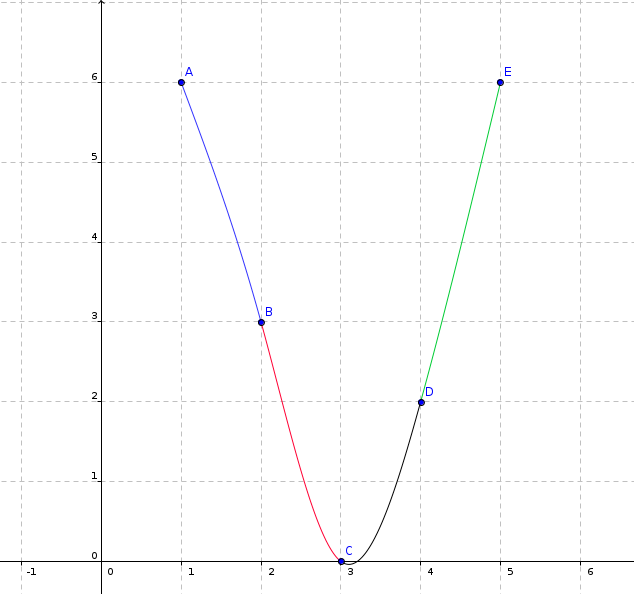
\includegraphics[width=8.5cm] {ExempleInterpolationGeogebra.png}
	\caption{Exemple d'interpolation par spline cubique sur Geogebra}
\end{figure}

\newpage
\subsection{Pr\'esentation de l'outil informatique}

Nous avons eu acc\`{e}s \`a un programme pascal permettant de calculer des splines en entrant le nombre de points que nous voulions raccorder ainsi que leurs coordonn\'{e}es respectives. Afin d'avoir une meilleur ergonomie et une meilleur lisibilit\'{e}, nous avons remani\'{e} le programme. \\ Voici donc le programme que nous avons utilis\'{e}.

\subsubsection{Analyse descendante}

\newpage
\begin{landscape}
\begin{figure}
	\centering
	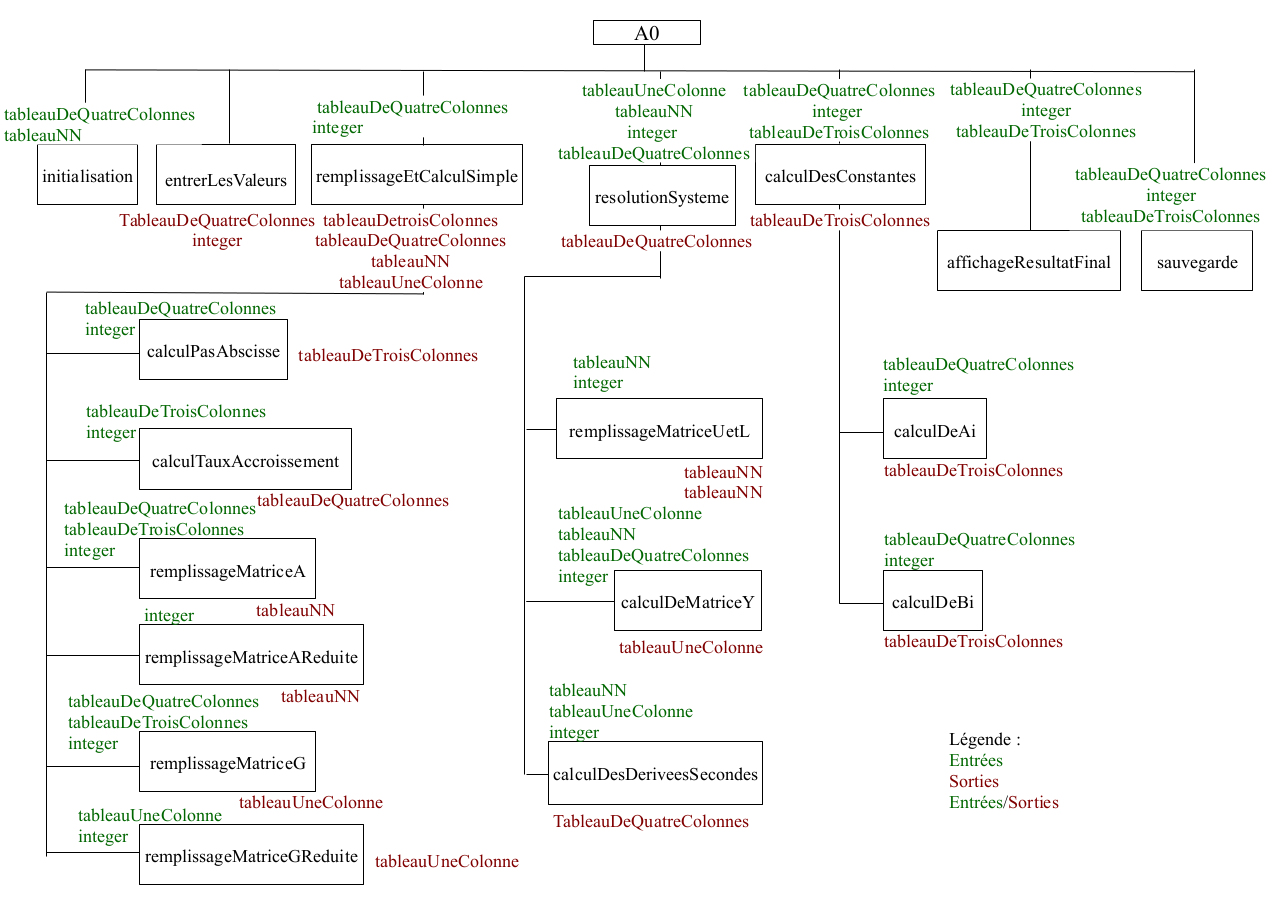
\includegraphics[width=20cm]{Analyse-Descendante-Spline-Cubique.png}
	\caption{Analyse descendante du programme}
\end{figure}
\end{landscape}


\newpage
\subsubsection{Pr\'esentation du contenu du programme}

\begin{enumerate}
	\item[o] \it Function fileExists (nomDuFichier : String) : Boolean;\\
	\rm Renvoie un bool\'{e}en vrai si le fichier existe.\\
	
	\item[o] \it Procedure sauvegarde (donneesAuPoint : tableauDeQuatreColonnes; nombrePoint : integer; donneesEntreDeuxPoints : tableauDeTroisColonnes);\\
	\rm Permet de sauvegarder les r\'{e}sultats du programme dans un fichier .txt dans le repertoire du fichier exc\'{e}cutable.\\
	
	\item[o] \it Procedure initialisation (Var donneesAuPoint : tableauDeQuatreColonnes; Var matriceA : tableauNN);\\
	\rm Initialise les tableaux \it donnesAuPoint \rm et \it matriceA \rm \`a z\'{e}ro.\\
	
	\item[o] \it Procedure entrerLesValeurs (Var donneesAuPoint : tableauDeQuatreColonnes; Var nombrePoint : integer);\\
	\rm Permet d'entrer le nombre de points et leurs coordonn\'ees respectives.\\
	
	\item[o] \it Procedure affichageResultatFinal (donneesAuPoint : tableauDeQuatreColonnes; nombrePoint : Integer; donneesEntreDeuxPoints : tableauDeTroisColonnes);\\
	\rm Affiche les r\'{e}sultats \`a l'\'{e}cran.\\
	
	\item[o] \it Procedure calculPasAbscisse (Var donneesEntreDeuxPoints : tableauDeTroisColonnes; donneesAuPoint : tableauDeQuatreColonnes ; nombrePoint : Integer); \\
	\rm La proc\'{e}dure calcule le pas, not\'e \it h \rm dans la r\'{e}solution math\'{e}matique entre les abscisses des points  $[x_{i},x_{i+1}]$.\\
	
	\item[o] \it Procedure calculTauxAccroissement (Var donneesAuPoint : tableauDeQuatreColonnes; donnesEntreDeuxPoints : tableauDeTroisColonnes; nombrePoint : Integer);\\
	\rm La proc\'{e}dure permet de calculer le taux d'accroissement \`a partir des valeurs entr\'ees.\\
	
	\item[o] \it Procedure remplissageMatriceA (Var matriceA : tableauNN; donneesAuPoint : tableauDeQuatreColonnes; donnesEntreDeuxPoints : tableauDeTroisColonnes; nombrePoint : integer);\\
	\rm Cette proc\'{e}dure simplifie le syst\`eme en le transposant dans une matrice.\\
	
	\newpage
	\item[o] \it Procedure remplissageMatriceAReduite (Var matriceA,matriceAR : tableauNN; nombrePoint : Integer);\\
	\rm Dans la matrice A initiale, on a plusieurs lignes compos\'{e}es de 1 et de 0. On peut donc r\'{e}duire la matrice aux lignes correspondantes aux valeurs des $f''_{i}$ non nulles. On r\'{e}\'{e}crit ainsi les lignes du "milieu" de la matrice A dans la matrice AR (A R\'{e}duite).\\
	
	\item[o] \it Procedure remplissageMatriceG (Var matriceG : tableauUneColonne; donneesAuPoint : tableauDeQuatreColonnes; donneesEntreLesPoints : tableauDeTroisColonnes; nombrePoint : Integer);\\
	\rm On a la matrice G r\'{e}sultante de A multipli\'{e}e par les d\'{e}riv\'{e}es secondes.\\
	
	\item[o] \it Procedure remplissageMatriceGReduite (Var matriceG, matriceGR : tableauUneColonne; nombrePoint : Integer);\\
	\rm On effectue le m\^eme principe qu'avec la matrice A pour la matrice G : On a des valeurs de $f''_{i}$ nulles. On r\'{e}duit alors la matrice G.\\
	
	\item[o] \it Procedure remplissageEtCalculSimple (Var donneesEntreDeuxPoints : tableauDetroisColonnes; Var donneesAuPoint : tableauDeQuatreColonnes; nombrePoint : Integer; Var matriceAR : tableauNN; Var matriceGR : tableauUneColonne); \\
	\rm Cette procedure appelle les proc\'{e}dures pr\'{e}c\'{e}dentes pour calculer le pas, le taux d'accroissement, les matrices A et G r\'{e}duites.\\
	
	\item[o] \it Procedure calculDeAi (donneesAuPoint : tableauDeQuatreColonnes; nombrePoint : Integer; Var donneesEntreDeuxPoints : tableauDeTroisColonnes);\\
	\rm On calcule ici les coefficients $a_{i}$.\\
	
	\item[o] \it Procedure calculDeBi (donneesAuPoint : tableauDeQuatreColonnes; nombrePoint : Integer; Var donneesEntreDeuxPoints : tableauDeTroisColonnes);\\
	\rm On calcule ici les coefficients $b_{i}$.\\
	
	\item[o] \it Procedure calculDesConstantes (donneesAuPoint : tableauDeQuatreColonnes; nombrePoint : Integer; Var donneesEntreDeuxPoints : tableauDeTroisColonnes);\\
	\rm Appelle les deux proc\'{e}dures pr\'{e}c\'{e}dentes : $calculDeAi \;$ et $calculDeBi$.\\
	
	\item[o] \it Procedure remplissageMatriceUetL (Var matriceL : tableauNN; Var matriceU : tableauNN; matriceAR : tableauNN; nombrePoint : Integer);\\
	\rm On cherche ici \`{a} d\'{e}composer A en deux matrices bidiagonales telles que A=UL.
	
	\item[o] \it Procedure calculDeMatriceY (Var matriceY, matriceGR : tableauUneColonne; matriceL : tableauNN; donneesAuPoint : tableauDeQuatreColonnes; nombrePoint : Integer);\\
	\rm Cette proc\'edure permet de calculer la matrice Y qui va \^etre multipli\'ee par L.\\
	
	\item[o] \it Procedure calculDesDeriveesSecondes (Var donneesAuPoint : tableauDeQuatreColonnes; matriceU : tableauNN; matriceY : tableauUneColonne; nombrePoint : Integer);\\
	\rm Cette proc\'{e}dure permet de calculer les d\'{e}riv\'{e}es secondes de $f$.\\
	
	\item[o] \it Procedure resolutionSysteme (matriceG :  tableauUneColonne; matriceA : tableauNN; nombrePoint : Integer; Var donneesAuPoint : tableauDeQuatreColonnes);\\
	\rm Ici, on appelle les proc\'{e}dures de remplissage de U et L, de calcul de la matrice Y et de calcul des d\'{e}riv\'{e}es pour r\'{e}soudre le syst\`eme.\\
\\
	Le programme principal ex\'{e}cute finalement les fonctions et les proc\'{e}dures pour calculer les fonctions splines cubiques. A l'ex\'{e}cution du programme, un r\'{e}pertoire nomm\'{e} \guillemotleft $\;$R\'{e}sultats \guillemotright $\;$est cr\'{e}\'{e} s'il n'existe pas encore, dans le r\'{e}pertoire o\`{u} se trouve le programme.\\

\end{enumerate}

\newpage
\section{B-splines}
\subsection{Contexte}
Les courbes de B\'ezier sont totalement modifi\'ees si un changement de point de contr\^ole est effectu\'e. Pour cette raison la m\'ethode de ces courbes peut \^etre qualifi\'ee de m\'ethode globale.\\
\indent
Les courbes de B-splines ont \'et\'e d\'efinies par Cox et De Boor dans les ann\'ees 1970 et d\'ev\'elopp\'ees par Boeing dans les ann\'ees 1980. Ils cherchaient un moyen pour utiliser les courbes de B\'ezier sans ces inconv\'enients. Boeing a donc remplac\'e les polyn\^omes de Berstein ($B_{i}^{k}$) par des fonctions de base des B-splines ($B_{i,k}$). Ainsi, les courbes de B-splines sont d\'etermin\'ees par ces fonctions de base, des points de contr\^ole et un vecteur n\oe ud.
Les courbes de B-splines sont stables num\'eriquement, ayant des coefficients toujours positifs. De plus elles sont faciles \`a interpr\'eter g\'eom\'etriquement. La variation d'un point de contr\^ole modifie seulement une partie limit\'ee de la courbe, ce qui repr\'esente un grand avantage pour la Conception Assist\'ee par Ordinateur. 
Alors, la m\'ethode de B-splines est consid\'er\'ee comme une m\'ethode locale.\\
\indent
De plus, les courbes de B-splines, \'etant \'equivalent \`aux courbes de B\'ezier continues sur $C^{2}$, sont les plus utilis\'ees dans l'interpolation des splines unidimensionnelles.\\
\\
\textbf{NURBS}\\
\indent
Les B-splines rationnelles non-uniformes, ou NURBS de leur acronyme anglais (\emph{Non-Uniform Rational Basis Splines}), donnent la possibilit\'e de repr\'esenter facilement des courbes qui ne peuvent pas \^etre construites par les B-splines uniformes. Les points de contr\^ole \'etant des rationnnels, l'utilisation de ces courbes permet de r\'eduire le nombre de noeuds d'une approximation tout en conservant une bonne pr\'ecision pour un arc ou une facette de courbe quelconque. \\
\indent
Apr\`es avoir effectu\'e toutes les transformations affines (translation, rotation, homoth\'eties) et aussi quelques transformations non isom\'etriques comme les projections ou la perspective, les NURBS conservent toutes ces propri\'et\'es, et m\^eme certaines caract\'eristiques physiques essentielles comme la continuit\'e, la pr\'eservation des tangentes ou angles aux sommets. \\
\indent
Gr\^ace \`a sa grande pr\'ecision, les NURBS sont utilis\'ees dans la cartographie. \'Etant compatibles avec la plupart des projections dans ce domaine, les NURBS interpolent des distances et des angles \`a partir d'un volume r\'eduit de mesures g\'eod\'esiques.\\
\indent
En outre, les NURBS sont une partie indispensable dans les syst\`emes de CAO les plus r\'ecents : ceci est d\^u \`a leur efficacit\'e et \`a leur pr\'ecision dans la repr\'esentation des images en 2 et 3 dimensions. Et  elles sont aussi exploit\'ees dans la majorit\'e des instruments de mesures de haute pr\'ecision comme les miroirs et lentilles utilis\'es en astronomie. \\
\indent
En conclusion, les B-splines et les NURBS sont les m\'ethodes d'interpolation les plus pr\'ecises, mais elles sont encore en d\'eveloppement.

\subsection{Les bases des B-splines}
On prend le vecteur n\oe ud $T=(t_{0},t_{1},...,t_{m})$ avec $t_{i} \leq t_{i+1}$, $i\in[0,m-1]$ et $m\in\Re$.
On choisit aussi les points de contr\^ole $P_{0}$, $P_{1}$, ..., $P_{m}$ et on note $P_{i}=\overrightarrow{OP_{i}} $.
On doit \'elaborer une courbe $X_{0}(t)$ avec 
$X_{0}(t_{i})=P_{i}$ pour tout $i\in[0,m]$. La courbe est alors d\'efinie par :
\begin{center}$X_{0}(t) =\sum\limits_{i=0}^n B_{i,0}(t) . P_{i}$ \end{center}

Par contre, les points obtenus \`a l'aide de cette fonction ne seront pas suffisants. En effet, la courbe sera discontinue (avec des sauts).
C'est pour cette raison que l'on cherche \`a approcher $X_{0}(t)$ par une courbe lin\'eaire par morceaux $X_{1}(t)$, o\`u $t$ varie de $t_{i}$ \`a $t_{i+1}$, qui relie les points $P_{i-1}$ et $P_{i}$.
\begin{center}$X_{1}(t) = (\dfrac{t_{i+1}-t}{t_{i+1}-t_{i}})P_{i-1}+ (\dfrac{t-t_{i}}{t_{i+1}-t_{i}})P_{i}$, pour $t\in [t_{i},t_{i+1}[$ (1)\end{center}
Donc on a :
\\$X_{1}(t_{i}) = P_{i-1}$ 
\\$X_{1}(t_{i+1}) = P_{i}$

Si $t_{0},...,t_{m}$ sont diff\'erents, alors $X_{1}(t)$ est continue et peut s'\'ecrire sous la forme: 
\begin{center}$X_{1}(t) =\sum\limits_{i=0}^n B_{i,1}(t) . P_{i}$ \end{center}

Mais $B_{i,1}(t)$ n'est pas d\'efinie. \\

D'o\`u, pour $t\in [0,m]$, l'\'equation (1) nous donne :
\begin{align*} 
X_{1}(t)  & = \sum\limits_{i} (\dfrac{t_{i+1}-t}{t_{i+1}-t_{i}}.1_{[t_{i},t_{i+1}[}.P_{i-1} + \dfrac{t-t_{i}}{t_{i+1}-t_{i}}.1_{[t_{i},t_{i+1}[}.P_{i})
\\[5pt]
& = \sum\limits_{i} \dfrac{t_{i+1}-t}{t_{i+1}-t_{i}}.1_{[t_{i},t_{i+1}[}.P_{i-1}+ \sum\limits_{i} \dfrac{t-t_{i}}{t_{i+1}-t_{i}}.1_{[t_{i},t_{i+1}[}.P_{i}
\end{align*} 

On pose $i' = i-1 $ pour la premi\`ere somme:
\begin{align*}
X_{1}(t) & = \sum\limits_{i'} (\dfrac{t_{i'+2}-t}{t_{i'+2}-t_{i'+1}}.1_{[t_{i'+1},t_{i'+2}[}.P_{i'})+ \sum\limits_{i} (\dfrac{t-t_{i}}{t_{i+1}-t_{i}}.1_{[t_{i},t_{i+1}[}.P_{i})
\\[5pt]
& = \sum\limits_{i} (\dfrac{t_{i+2}-t}{t_{i+2}-t_{i+1}}.1_{[t_{i+1},t_{i+2}[} + \dfrac{t-t_{i}}{t_{i+1}-t_{i}}.1_{[t_{i},t_{i+1}[}).P_{i}
\\[5pt]
& = \sum\limits_{i} (\dfrac{t_{i+2}-t}{t_{i+2}-t_{i+1}}.B_{i+1,0}(t) + \dfrac{t-t_{i}}{t_{i+1}-t_{i}}.B_{i,0}(t)).P_{i}
\end{align*}

Alors:

\begin{center}$B_{i,1}(t) = \dfrac{t_{i+2}-t}{t_{i+2}-t_{i+1}}.B_{i+1,0}(t) + \dfrac{t-t_{i}}{t_{i+1}-t_{i}}.B_{i,0}(t)$
\end{center}


Donc la fonction de degr\'e 1, $X_{1}(t) =\sum\limits_{i=0}^n B_{i,1}(t) . P_{i}$ est d\'efinie en utilisant  $X_{0}(t) =\sum\limits_{i=0}^n B_{i,0}(t) . P_{i}$, de degr\'e 0. De la m\^eme fa\c con, en g\'en\'eralisant, on trouve: 

\begin{center}$X_{k}(t) =\sum\limits_{i} B_{i,k}(t) . P_{i}$ \end{center}

les $P_{i}$ \'etant les points de contr\^ole de la courbe. Il y a \'evidemment le m\^eme nombre de $B_{i,k}$ que de $P_{i}$ soit de $P_{0}$ \`a $P_{n}$ . Le vecteur n\oe ud $(t_{0} , t_{1} , ..., t_{m})$ sera tel que $m=n+k+1$ \'etant donn\'e que les $B_{i,k}$ s'\'etalent sur $k + 1$ n\oe uds et 
 
\begin{center}$B_{i,k}(t)= \dfrac{t_{i+1+k}-t}{t_{i+1+k}-t_{i+1}}B_{i+1,k-1}(t) + \dfrac{t-t_{i}}{t_{i+k}-t_{i}}B_{i,k-1}(t)$ \end{center}

$B_{i,k}(t)$ est une fonction de base d'une B-spline, qui est g\'{e}n\'{e}ralement appel\'{e}e \textbf{base de B-splines}.

Dans la partie qui suit, on va s'int\'{e}resser aux B-splines de degr\'{e} 3, bien que les d\'{e}marches soient g\'{e}n\'{e}ralisables.


\subsection{Courbe de degr\'ee 3 (k=3)}

Si on veut placer $n$ points de contr\^ole, on doit d\'{e}terminer $n+4$ n\oe uds. Il nous faut aussi un vecteur n\oe ud. Par exemple, on prend le vecteur $(1,2,3,4,5,6,7)$ et on d\'{e}finit les points de contr\^ole $(1,1),(1,3),(2,4),(3,1)$. Apr\`es des calculs et en variant $t$ de $0$ \`a $7$, on obtient la courbe en rouge. On remarque que cette courbe a une forme particuli\`ere. Elle commence et finit \`a l'origine du rep\`{e}re et elle ne passe pas par le premier et le dernier point de contr\^ole. Cela peut s'expliquer par le fait que, en $t=0$ et en $t=7$, les $B_{i,3}$ sont nulles et par cons\'{e}quent la courbe de B-splines est aussi nulle. De plus, pour \'eviter cet inconv\'{e}nient, on fait varier $t$ entre $3$ et $4$ tel que $B_{i,3}$ est \'{e}gale \`a 1. On obtient la partie de la courbe color\'{e}e en vert, qui est relativement plus proche de la courbe mod\'{e}lis\'{e}e en bleu par les points de contr\^ole $P_{0}$ \`a $P_{3}$.

\begin{figure}[h]
	\centering
	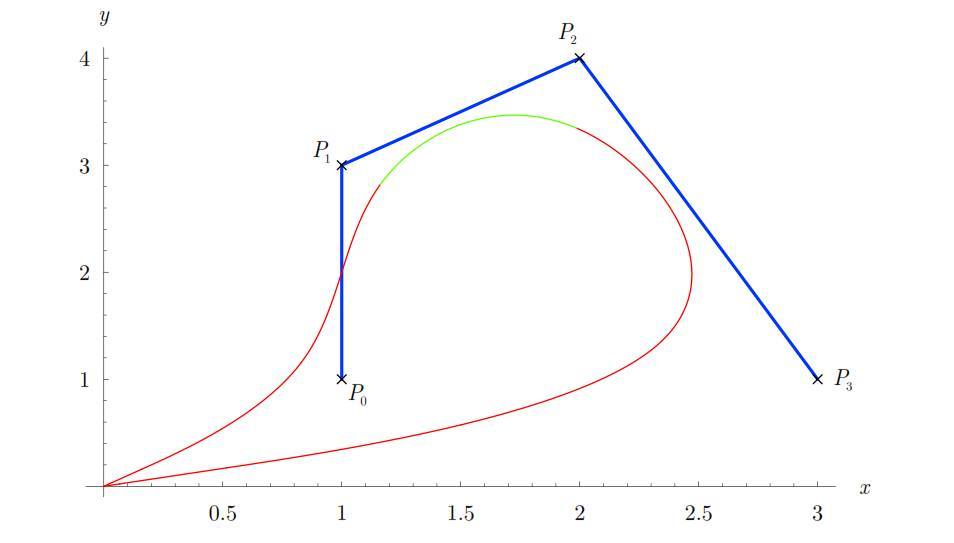
\includegraphics[width=11cm]{Courbe-B-splines.jpg}
	\caption{Courbe de B-spline de degr\'e 3 }
\end{figure}

\textbf{R\'{e}p\'{e}tition des n\oe uds}
On peut, sans probl\`eme, r\'{e}p\'{e}ter des n\oe uds si on veut que la courbe passe par un point pr\'{e}cis. Pour les n\oe uds internes, il suffit par exemple de r\'{e}p\'{e}ter le point trois fois pour le degr\'{e} 3 (soit $k=3$). Pour les points extr\^{e}mes, il faut encore une r\'{e}p\'{e}tition et ce ph\'{e}nom\`{e}ne s'appelle B-splines \`a n\oe ud ouvert. Par contre, avec cette action, la fonction de la courbe n'est plus d\'{e}rivable, ce qui s'explique par le fait qu'une fonction de base $B_{i,k}$ est d\'{e}rivable $k-r$ fois, o\`u $r$ est la multiplicit\'{e} d'un point. 

\textbf{R\'{e}p\'{e}tition des points de contr\^ole }
La r\'{e}p\'{e}tition des points 3 fois implique aussi que la courbe passe par un point pr\'{e}cis.
Par exemple, en prenant $8$ n\oe uds distincts et en choisissant $P_{1} = P_{2} = P_{3}$, on calcul $X_{3}(t_{4})$:

\begin{center}$X_{3}(t_{4}) = B_{1,3}.P_{1} + B_{2,3}.P_{2} + B_{3,3}.P_{3} $
\end{center}

Les autres bases $B_{4,3}$, $B_{5,3}$, ... ne figurent pas dans la formule car en $t_{4}$, elles sont \'{e}gales \`a $0$. 

\begin{center}$X_{3}(t_{4}) = ( B_{1,3} + B_{2,3} + B_{3,3}).P_{1} $
\end{center}

O\`u $B_{1,3} + B_{2,3} + B_{3,3} = 1$, donc $X_{3}(t_{4}) = P_{1}$

Par contre, la fonction de la courbe reste ind\'{e}rivable apr\`{e}s la r\'{e}p\'{e}tition des points.

\subsection{Contr\^ole local}
\textbf{Modification d'un point de contr\^ole }
(exemple pour k = 3) Le fait de changer un point de contr\^ole  $P_{i}$ modifie la courbe seulement entre $t_{i}$ et $t_{i+4}$.

\textbf{Modification d'un n\oe ud}
Le changement d'un n\oe ud ne fait varier que les $B_{i,k}$ autour. Pour $k = 3$, les fonctions des courbes modifi\'{e}es varient entre les bases $B_{i-4,k}$ et $B_{i,k}$ (ce qui n'est pas valable pour les extr\'{e}mit\'{e}s) et modifie les $t$ de $t_{i-4} $ \`a $t_{i+4} $.


\subsection{Autres propri\'et\'es}
Les B-Splines on beaucoup d'autres propri\'{e}t\'{e}s dont:
\\- la diff\'{e}rentiabilit\'{e} des B-Splines;
\\- l'ajout d'un n\oe ud sans modifier la courbe;
\\- l'\'{e}l\'{e}vation du degr\'{e} sans changer la courbe;
\\- la sym\'{e}trie des points de contr\^ole impliquant une courbe sym\'{e}trique.

\newpage
\subsection{Pr\'esentation de l'outil informatique}
\begingroup\raggedleft
Les commentaires de ce programme se trouvent dans le fichier bspline.pas.
Programme B-splines
\endgroup
\\
Signatures :
\begin{itemize}
\item [o] Function BI0 (I:Integer; X:Real):Real ;
\item [o] Function BI1 (I:Integer; X:Real):Real ;
\item [o] Function BI2 (I:Integer; X:Real):Real ;
\item [o] Function BI3 (I:Integer; X:Real):Real ;
\item [o] Function Bspline (N:Integer; A:Tabulation; X:Real): Real ;
\item [o] Procedure TraceBspline (A:Tabulation; N:Integer; X0, X1: Real) ;
\item [o] Procedure CalculCoeff (N:Integer; var A:Tabulation) ;
\item [o] Procedure Init (NP, C:Integer; XD, XF:Real) ;
\end{itemize}

\begin{figure}[h]
	\centering
	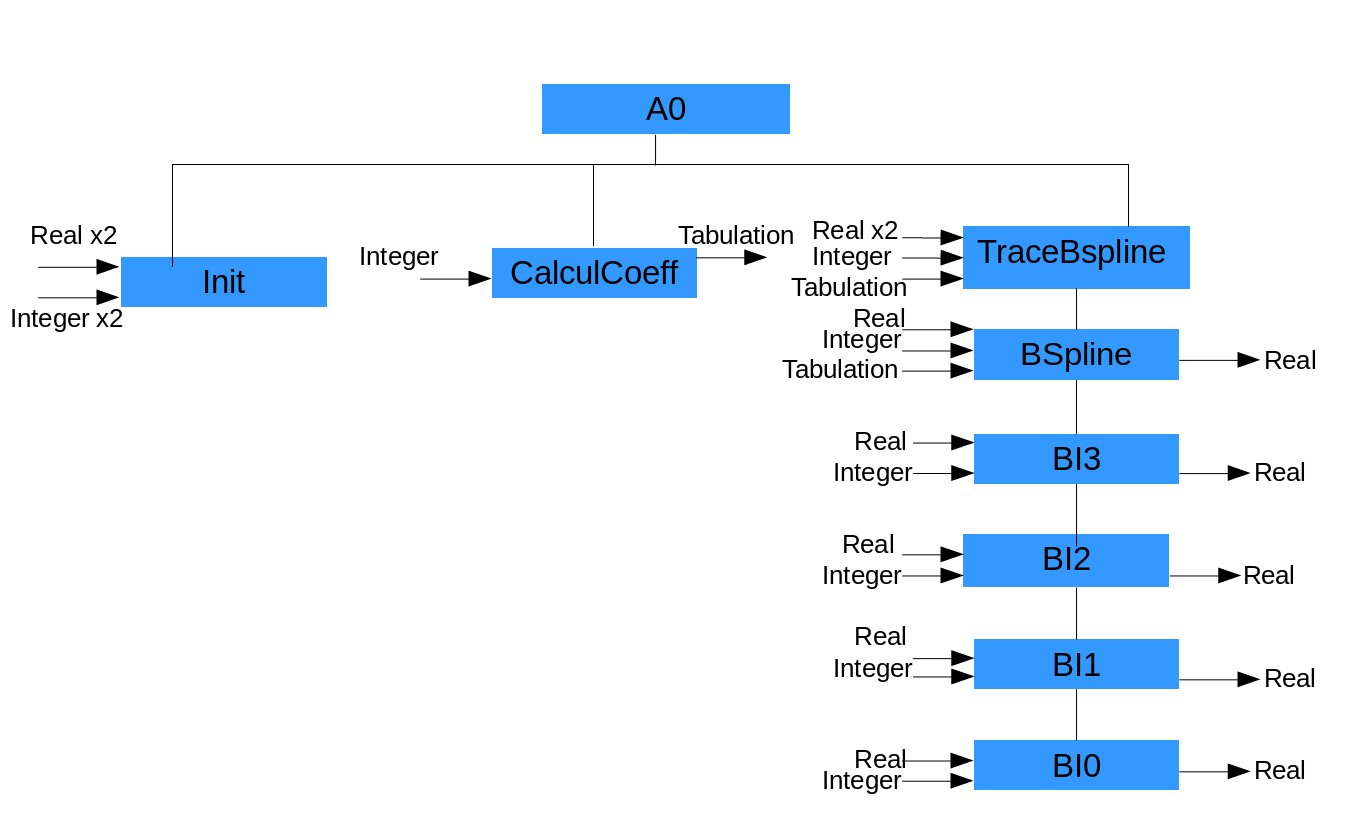
\includegraphics[width=15cm]{Analyse-Descendante-bspline.png}
	\caption{Analyse descendante du programme}
\end{figure}

\newpage
\section{Avantages et inconv\'{e}nients}
\subsection{Courbes de B\'{e}zier : avantages et inconv\'{e}nients}

\begin{flushleft}
AVANTAGES :
\end{flushleft}
\par
Les courbes de B\'{e}zier pr\'{e}sentent de nombreux avantages mais aussi des inconv\'{e}nients que nous allons pr\'{e}senter afin de comprendre l'\'{e}volution vers les splines cubiques.
Utilisant des polyn\^{o}mes de degr\'{e}s assez petits, les courbes de B\'{e}zier sont faciles \`{a} calculer et \`{a} tracer sans que cela nuise pour autant \`{a} la complexit\'{e} des formes g\'{e}om\'{e}triques repr\'{e}sent\'{e}es. Il est en effet possible de d\'{e}crire des formes \'{e}l\'{e}mentaires vari\'{e}es comme des courbes concaves ou convexes, des inflexions, n\oe{}uds ou rebroussements, formes non repr\'{e}sentables \`{a} l'aide d'un polygone.
Une particularit\'{e} importante des courbes de B\'{e}zier concerne la m\'{e}thode de tra\c{c}age. Cette technique utilise des points de contr\^{o}le et non des points d'interpolation ainsi la courbe ne passe pas par les points donn\'{e}s-comme c'est le cas pour les interpolations- mais les approche. Cette approximation poss\`{e}de plusieurs avantages :
\\
- les points de contr\^{o}le guident g\'{e}om\'{e}triquement la courbe, ce qui permet d'obtenir plus facilement une courbe d'aspect naturel.
\\
- Il est possible de pr\'{e}voir les d\'{e}formations des courbes gr\^ace \`{a} sa stabilit\'{e} satisfaisante.
\\
- La courbe est facile \`{a} modifier en d\'{e}pla\c{c}ant les points de contr\^{o}le qui sont peu nombreux. Les agrandissements, d\'{e}formations et toutes les transformations que l'on peut r\'{e}aliser sur un polyn\^{o}me (rotation, translation, mise \`{a} l'\'{e}chelle, inclinaison...) sont ainsi applicables.
\\\\
INCONVENIENTS :
\\
\par
Malheureusement, les courbes de B\'{e}zier poss\`{e}dent aussi des inconv\'{e}nients non n\'{e}gligeables.
Ces courbes ont un contr\^{o}le global et manquent de contr\^{o}le local. La modification d'un point fait bouger toute la courbe, ce qui est probl\'{e}matique dans des domaines tels que l'industrie automobile : il est g\^{e}nant que toute la pi\`{e}ce change de forme lorsque nous voulons seulement faire varier une partie de la pi\`{e}ce. Au niveau des calculs, il faudra calculer \`{a} nouveau toute la pi\`{e}ce.
La courbe ne passant pas par les points de contr\^{o}le, il est difficile de la contr\^{o}ler pr\'{e}cis\'{e}ment.
Pour r\'{e}aliser une forme complexe, les courbes de B\'{e}zier n\'{e}cessitent beaucoup de points de contr\^{o}le et donc des degr\'{e}s de courbe plus \'{e}lev\'{e}s ce qui les rend difficile \`{a} manipuler. 
La fonction de Runge mets en \'{e}vidence ce dernier point. L'interpolation polynomiale n'est pas adapt\'{e}e \`{a} l'approximation de fonctions pour grand n.

\newpage
\subsection{Splines cubiques : avantages et inconv\'{e}nients}

\begin{flushleft}
AVANTAGES
\end{flushleft}
\par
Les principaux avantages de l'interpolation par spline sont sa stabilit\'{e} et simplicit\'{e} de calcul.
Une spline cubique \'{e}tant une fonction obtenue \`{a} l'aide de divers polyn\^{o}mes de degr\'{e}s inf\'{e}rieurs ou \'{e}gaux \`{a} 3. Ceci permet de limiter l'augmentation du degr\'{e} du polyn\^{o}me et ainsi \'{e}viter le ph\'{e}nom\`{e}ne de Runge (probl\`{e}me d'oscillation de Lagrange non pr\'{e}sent). En effet, lorsque l'on augmente n, cela augmente le nombre de morceaux et non le degr\'{e} des polyn\^{o}mes.
De plus, les faibles degr\'{e}s d'interpolation facilitent l'impl\'{e}mentation, ce qui les rend tr\`{e}s populaires.
En utilisant des morceaux de polyn\^{o}mes pour relier les points, on am\'{e}liore aussi la stabilit\'{e} de la courbe : le changement d'un point n'influence pas toute la courbe. Cet avantage est tr\`{e}s important pour les utilisations pratiques, il comble le d\'{e}faut principal des courbes de B\'{e}zier (manque de contr\^{o}le local).
Pour finir, les courbes sont harmonieuses, sans pointe ni d\'{e}tour... Les interpolations par splines cubiques sont donc tr\`{e}s utilis\'{e}es dans le domaine du design pour approcher des contours complexes sans avoir de cassure du rayon de courbure.
\\\\
INCONVENIENTS :
\\
\par
Avec l'interpolation par spline cubique, nous devons toutefois faire face \`{a} deux inconv\'{e}nients : la spline peut elle aussi devenir oscillante si les d\'{e}riv\'{e}es de la fonction \`{a} interpoler deviennent trop grandes (>>1) et sa r\'{e}solution est un peu plus complexe.

\subsection{B-splines : avantages et inconv\'{e}nients}

\begin{flushleft}
AVANTAGES :
\end{flushleft}
\par
Comme les splines cubiques, les B-splines r\'{e}solvent les probl\`{e}mes que nous avons constat\'{e} pour les courbes de B\'{e}zier. Le contr\^{o}le local est possible pour les B-splines et l'ajout de points n'augmente pas le degr\'{e} de la courbe. Nous pouvons ajouter que le degr\'{e} du polyn\^{o}me est ind\'{e}pendant du nombre de points de contr\^{o}le.
\\\\
INCONVENIENTS :
\\
\par
Le principal inconv\'{e}nient des B-splines est leur complexit\'{e}. En effet, il n'est pas facile de calculer les fonctions de base. Les points de contr\^{o}le ne sont plus les seuls param\`{e}tres des courbes, il y a aussi le vecteur n\oe{}ud. Il est difficile de g\'{e}rer les points et les n\oe{}uds en m\^{e}me temps. C'est pourquoi nous ne faisons que varier les points de contr\^{o}le, les n\oe{}uds sont g\'{e}n \'{e}ralement ouverts aux extr\'{e}mit\'{e}s et uniformes au milieu.

\newpage
\begin{huge}
\section{Exemples de fonctions}
\end{huge}

\begin{huge}
\subsection{Fonction de Runge}
\end{huge}
\begin{huge}
\subsubsection{Introduction} 
\end{huge}

La logique des interpolations consiste \`{a} ce que, plus on augmente le nombre de noeuds d'interpolation, plus la courbe trac\'{e}e sera pr\'{e}cise. Or, en 1901, Carle David Tolme Runge, math\'{e}maticien allemand, a \'etudi\'e un r\'{e}sultat diff\'{e}rent : il s'agit du ph\'{e}nom\`{e}ne de Runge, associ\'{e} \`a sa fonction, qui se retrouve dans le cas de l'interpolation polynomiale de Lagrange. En effet, aux bords d'un intervalle d'interpolation, des oscillations, ne correspondant pas \`a la fonction recherch\'{e}e, peuvent appara\^itre. Ces oscillations augmentent avec le degr\'{e} du polyn\^ome d'interpolation mais il y a tout de m\^eme convergence du polyn\^ome vers la fonction sur un intervalle r\'{e}duit par rapport au domaine d\'{e}fini initialement.

\begin{huge}
	\subsubsection{Exemple} 
\end{huge}
Nous nous sommes int\'{e}ress\'{e}s \`a la fonction de Runge, c'est \`a dire \`a $f(x)=\frac{1}{1+25x^{2}}$. Nous voulons \'{e}tudier l'allure de cette fonction sur l'intervalle [-1;1]. Pour cela, nous avons trac\'{e} la fonction sur Open Office Excel \`a l'aide des points suivants:

\begin{figure}[h]
	\centering
	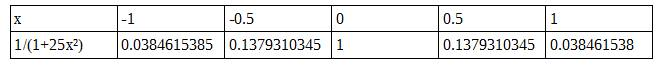
\includegraphics[width=8cm]{TableauDeValeurs.png}
	\caption{Tableau de r\'{e}sultats de la fonction de Runge en fonction des valeurs de x}
\end{figure}

\vspace{2\baselineskip}

\begin{figure}[h]
	\centering
	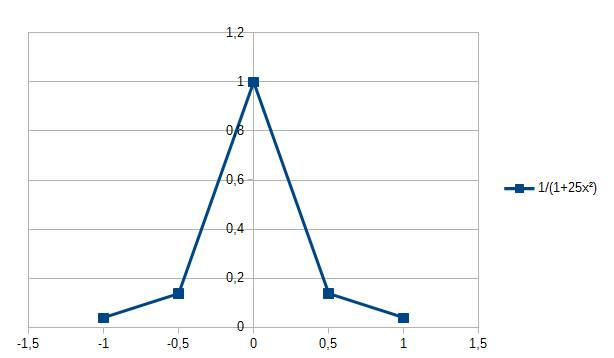
\includegraphics[width=10cm]{CourbeFonctionRunge.png}
	\caption{Repr\'{e}sentation graphique de la fonction de Runge sur l'intervalle [-1;1] }
\end{figure}

\newpage
La courbe obtenue \`a l'aide d'un tableur est une succession de segments de droites donc tr\`{e}s lin\'{e}aire et n'a pas l'allure lisse et courb\'{e}e attendue de la fonction Runge. 

Pour comparer, nous avons utilis\'{e} les m\^{e}mes coordonn\'{e}es de points dans notre programme FonctionSplineCubique, que  nous avons modifi\'{e} afin d'y mettre des fractions ($\frac{1}{26}$ dans notre cas). Apr\`es avoir obtenu une s\'{e}rie de fonctions splines, nous avons trac\'{e} la courbe correspondante sur le logiciel Geogebra. 

\begin{figure}[h]
	\centering
	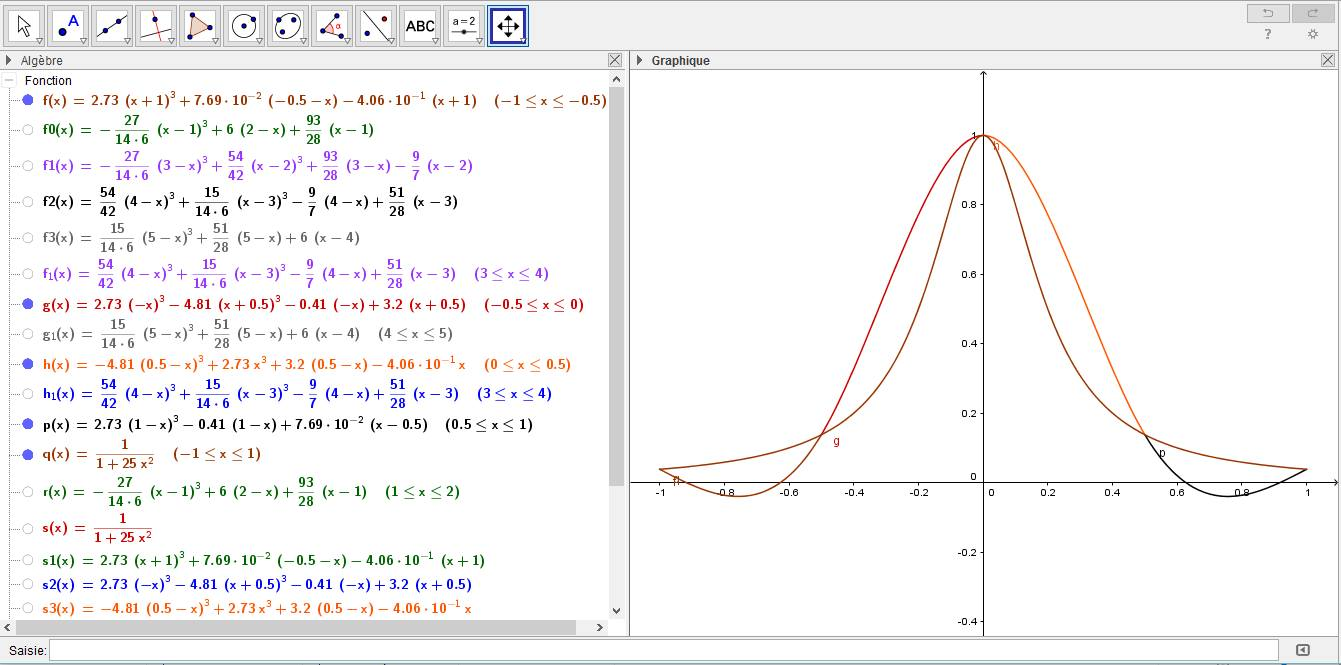
\includegraphics[width=12cm]{InterpolationRungeSplineCubique.png}
	\caption{Repr\'{e}sentation graphique de l'interpolation de la fonction de Runge par spline cubique }
\end{figure}

\newpage
Nous obtenons alors une courbe bien plus lisse. On remarque que vers le milieu de l'intervalle de d\'{e}finition, la fonction d'interpolation se rapproche de la fonction recherch\'{e}e mais que le ph\'{e}nom\`ene de Runge est pr\'{e}sent aux extr\'{e}mit\'{e}s de l'intervalle, comme expliqu\'{e} pr\'{e}c\'{e}demment.

Voici une autre repr\'{e}sentation de cette m\^{e}me fonction avec 10 puis 20 n\oe uds d'interpolation :

\begin{figure}[h]
	\centering
	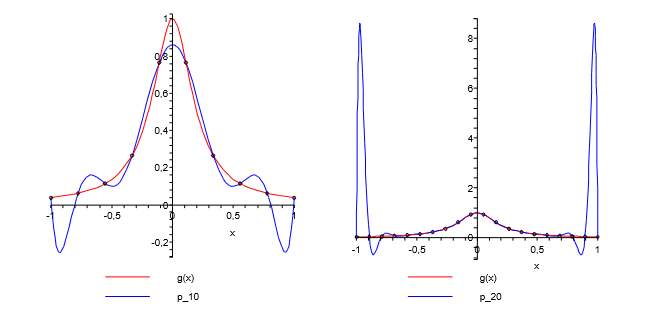
\includegraphics[width=12cm]{ExempleFctRunge.png}
	\caption{Repr\'{e}sentation graphique du ph\'{e}nom\`{e}ne de Runge visible aux extr\'{e}mit\'{e}s de l'intervalle de d\'{e}finition }
\end{figure}

Ce ph\'{e}nom\`{e}ne de Runge n'appara\^it pas dans tous les cas (comme par exemple avec $f(x)=\frac{1}{1+x^{2}}$) et peut \^{e}tre att\'{e}nu\'{e} par l'utilisation de courbes B-splines.\\

\newpage
\subsection{Fonction Cosinus} 

A titre de second exemple, nous nous sommes int\'{e}ress\'{e}s \`a la fonction
cosinus. Initialement, nous avions pr\'{e}vu de la tracer sur l'intervalle $[0; \pi]$, mais la fonction \'{e}tant impaire sur le point $(\pi/2 ; 0)$, nous nous sommes limit\'{e}s \`a l'intervalle $[0; \pi/2]$.\\

\begin{center}
\begin{table}[!hbp]
\begin{center}
\begin{tabular}{|c|c|c|c|c|c|}
\hline
\hline
 x & 0 & 0.3927 & 0.7854 & 1.1781 & 1.5708 \\
\hline
 cos(x) & 1 & 0.9239 & 0.7071 & 0.3827 & 0 \\
\hline
\end{tabular}
\end{center}
\end{table} 
\end{center}

\begin{figure}[h]
	\centering
	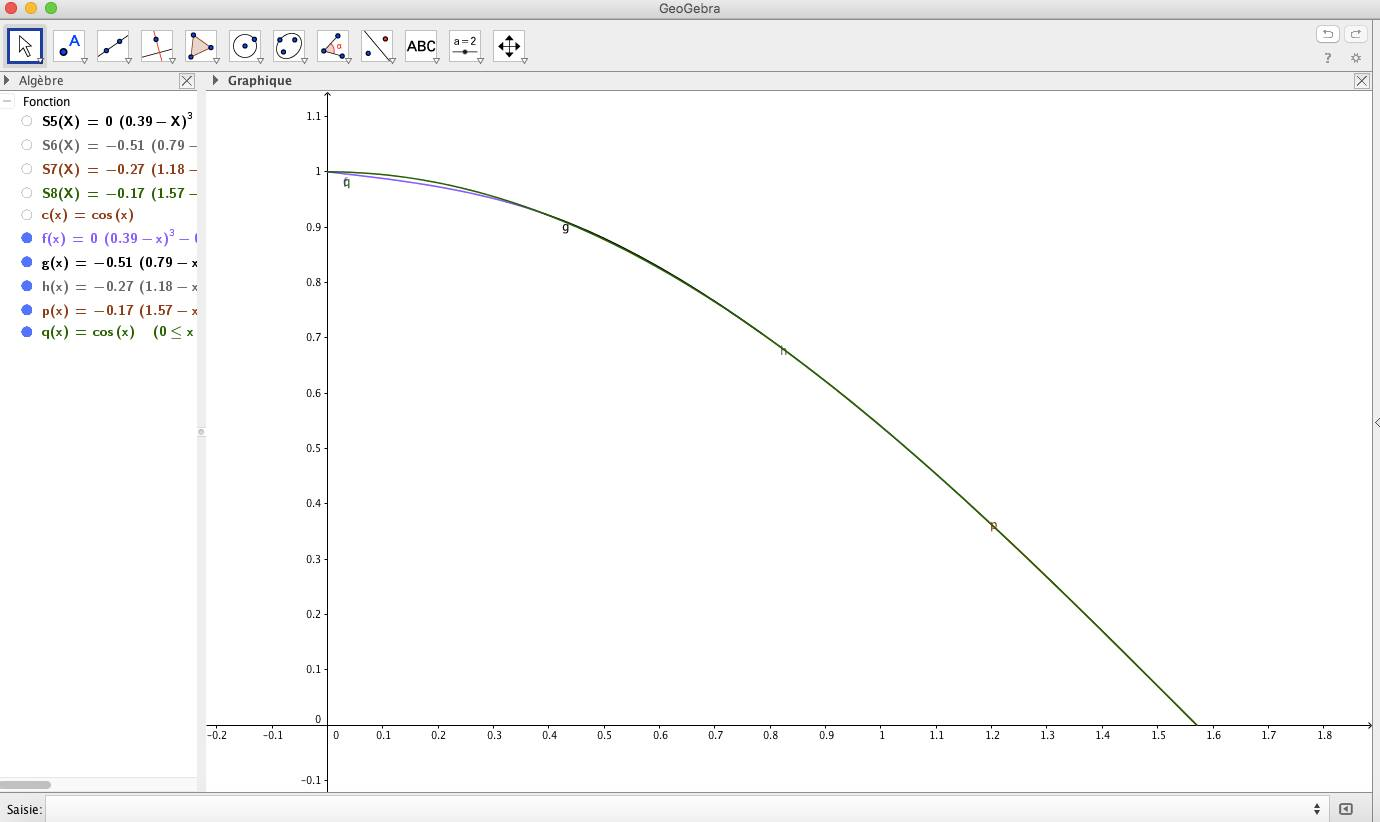
\includegraphics[width=8cm]{FonctionCosinus.jpg}
	\caption{Mod\'{e}lisation de la fonction Cosinus par spline cubique}
\end{figure}

L\`a encore, la fonction n'a pas l'allure attendue, elle n'est pas lisse et a un aspect quelque peu lin\'{e}aire.
De m\^{e}me que pour la fonction de Runge, en utilisant notre programme FonctionSplineCubique, nous avons relev\'{e} les m\^{e}mes coordonn\'{e}es puis utilis\'{e} les splines obtenues pour tracer la courbe sur GeoGebra.\\

\newpage

\subsection{Fonction Exponentielle} 

Nous nous sommes finalement int\'{e}ress\'{e}s \`a la fonction exponentielle mod\'{e}lis\'{e}e par une interpolation polynomiale. 
Nous avons tout d'abord d\'{e}cid\'{e} d'\'{e}tudier cette fonction avec Open Office Excel sur l'intervalle [-1;3], sans utiliser d'interpolation.\\

\begin{center}
\begin{table}[!hbp]
\begin{center}
\begin{tabular}{|c|c|c|c|c|c|}
\hline
\hline
 x & -1 & 0 & 1 & 2 & 3 \\
\hline
 exp(x) & 0.3679 & 1 & 2.7183 & 7.3891 & 20.0855 \\
\hline
\end{tabular}
\end{center}
\end{table} 
\end{center}

\begin{figure}[h]
	\centering
	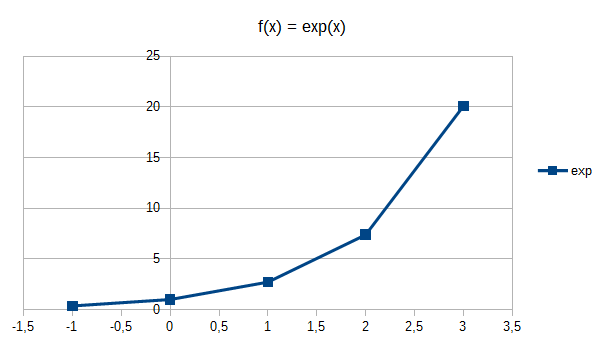
\includegraphics[width=12cm]{FctExpExcel.png}
	\caption{Repr\'{e}sentation graphique de la fonction exponentielle sur l'intervalle [-1;3] }
\end{figure}

La courbe obtenue \`a l'aide du tableur est une succession de segments de droite, elle est donc lin\'{e}aire. Mais elle a tout de m\^{e}me une allure assez proche de la fonction exponentielle recherch\'{e}e.\\
Ensuite, pour comparer, nous avons appliqu\'{e} la m\'{e}thode en utilisant cette fois le logiciel Geogebra. On a ainsi mod\'{e}lis\'{e} la fonction exponentielle \`a l'aide de quatre n\oe uds, r\'{e}partis sur l'intervalle [0;2].

\begin{figure}[h]
	\centering
	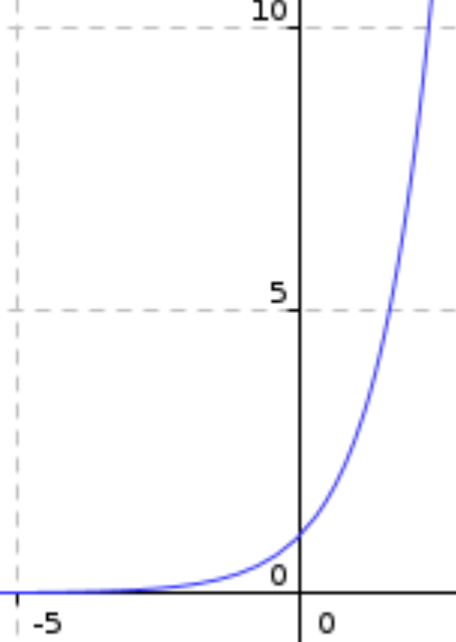
\includegraphics[width=5cm]{FonctionExponentielle.png}
	\caption{Nouvelle repr\'{e}sentation graphique de la fonction exponentielle sur l'intervalle [-1;3] avec Geogebra}
\end{figure}

\newpage

On retrouve une courbe \`a l'allure lisse comme celle de la fonction exponentielle. Les n\oe uds dans l'intervalle [0;2] sont confondus avec la courbe.\\\\\\\\\\\\\

Par cons\'{e}quent, nous nous sommes servis de trois exemples de fonctions usuelles afin de r\'{e}v\'{e}ler la pr\'{e}cision de la fonction d'interpolation par spline dans le tra\c cage de diff\'{e}rentes courbes de fonctions. En effet, \`a l'aide de notre programme FonctionSplineCubique, nous avons obtenu une s\'{e}rie de fonctions splines puis, \`a l'aide du logiciel GeoGebra, nous avons utilis\'{e} ces fonctions pour tracer les courbes. Nous avons ainsi pu retrouver une courbure fid\`{e}le \`a l'allure attendue des fonctions de Runge, cosinus et exponentielle dont l'aspect lisse provient des propri\'{e}t\'{e}s de l'interpolation par splines cubiques.\\

\newpage

\begin{huge}
\section{Applications des splines cubiques}
\end{huge}

Comme la partie historique de ce dossier le souligne, l'interpolation est un vieil outil math\'{e}matique. Son anciennet\'{e} nous montre qu'elle est utile \`a toute les \'{e}poques. En effet, l'interpolation permet de d\'{e}duire une infinit\'{e} de points \`a partir de seulement quelques mesures, ce qui est infiniment utile dans tous les m\'{e}tiers scientifiques. 
Si l'interpolation est d'une aussi grande utilit\'{e}, l'interpolation par spline l'est a fortiori puisqu'il s'agit d'une des m\'{e}thodes d'interpolations pr\'{e}sentant la plus petite erreur et le moins de d\'{e}viation. Comme le dit Thomas Grandine de la RD de Boeing : \guillemotleft  les splines sont tr\`{e}s utilis\'{e}es chez Boeing ainsi que dans la plus grande part du monde industriel. Il y a tr\`{e}s peu de domaines o\`u ces fonctions n'ont pas encore eu de r\^ole, et leur utilisation continue \`a s'intensifier.\guillemotright
\\Depuis le d\'{e}but de son d\'{e}veloppement dans les ann\'{e}es 50, celle-ci a connu de nombreuses applications dans des domaines vari\'{e}s. Etant limit\'{e}s par le temps (et la consid\'{e}ration \'{e}cologique du nombre de pages \`a imprimer bien s\^ur !) nous pr\'{e}senterons dans cette section une liste non exhaustive de ces domaines. Nous passerons bien \'{e}videmment par l'automobile mais aussi la typographie, la chimie, l'a\'{e}ronautique et le domaine de l'imagerie m\'{e}dicale.\\\\

\newpage
\begin{huge}
\subsection{Les splines dans la typographie et les logiciels de dessin}
\end{huge}

Une nouvelle application des splines cubiques est apparue avec l'arriv\'{e}e des ordinateurs. On les retrouve en typographie et plus pr\'{e}cis\'{e}ment, ils sont \`a la base des diff\'{e}rentes polices de caract\`{e}re que l'on trouve dans les traitements de texte. Par exemple, le Postscript est un langage informatique et de programmation complexe, cr\'{e}\'{e} dans les ann\'{e}es 1980, qui permet de communiquer avec les imprimantes. Les polices de caract\`{e}re en Postscript sont d\'{e}finies par des courbes de B\'{e}zier mais il n'y a pas d'interaction homme-machine comme pour les traitements de texte. On ne se rend donc pas compte que ce langage est utilis\'{e}.\\

La photo ci-dessous montre \`a gauche, la lettre \guillemotleft \ e \guillemotright \ grossie par un ordinateur des ann\'{e}es 80, et \`a droite, la m\^{e}me lettre avec un ordinateur d'aujourd'hui. La m\'{e}thode des splines cubiques est utilis\'{e}e pour cette derni\`{e}re.

\begin{figure}[h]
	\centering
	
\includegraphics[width=6cm]{Typographie.png}
	\caption{La lettre e avec un ordinateur des ann\'{e}es 80 (gauche) et un ordinateur d'aujourd'hui (droite)}
\end{figure}

La m\'{e}thode des splines cubiques permet, lorsque l'on agrandit ou diminue la taille de la police, de supprimer le ph\'{e}nom\`{e}ne de \guillemotleft \ pixellisation \guillemotright. On remarque alors que les lettres d'aujourd'hui sont plus lisibles, plus agr\'{e}ables \`a lire que celles d'il y a 30 ans. Il est \'{e}galement possible d'\'{e}crire la m\^{e}me lettre de  diff\'{e}rentes fa\c cons en raison des tr\`{e}s nombreuses polices existantes.\\

Avec le d\'{e}veloppement de l'informatique, cette application s'est aussi \'{e}tendue aux logiciels de dessin (mod\'{e}lisation), tels que Paint ou Geogebra. Les courbes de B\'{e}zier et les B-Splines sont utilis\'{e}es afin de mod\'{e}liser toutes les formes,  principalement g\'{e}om\'{e}triques, souhait\'{e}es. 

\newpage

\begin{figure}[h]
	\centering
	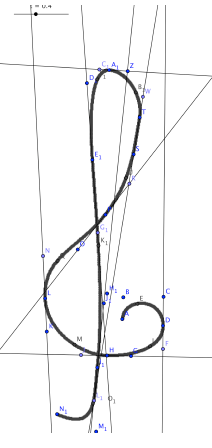
\includegraphics[width=3cm]{ClefSol.png}
	\caption{Dessin (\`a l'aide de B-splines) r\'{e}alis\'{e} par ordinateur avec le logiciel Geogebra.}
\end{figure}

Les points bleus visibles sur l'image repr\'{e}sentent les noeuds d'interpolation.\\

Cette m\'{e}thode s'est ensuite appliqu\'{e}e dans les logiciels de C.A.O. (Conception Assist\'{e}e par Ordinateur) ou dans le domaine du design. Nous expliquerons cela dans la partie qui suit.

\newpage
\begin{huge}
\subsection{Les splines dans les transports : l'a\'eronautique et l'automobile}
\end{huge}

Avant l'av\`{e}nement de l'ordinateur et des splines, il fallait utiliser d'autres moyens pour trouver une courbe lisse passant par des points donn\'{e}es. La photo ci-contre montre un ing\'{e}nieur de chez Boeing, dans les ann\'{e}es avant l'essort de l'ordinateur, en plein processus de cr\'{e}ation. Il utilise ce que les anglosaxons appelent un \guillemotleft \ draftsman's spline \guillemotright (une corde reli\'{e}e \`a des poids qui permettent de lui donner une forme). D'autres m\'{e}thodes consistaient par exemple en l'utilisation de r\`{e}gles flexibles. La photo ci-contre illustre bien la p\'{e}nibilit\'{e} de ce travail et nous donne une id\'{e}e du temps de travail n\'{e}cessaire.\\\\

\begin{figure}[h]
	\centering
	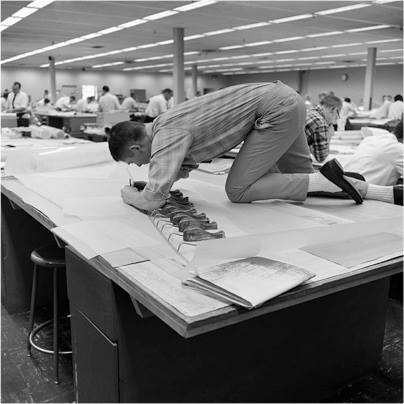
\includegraphics[width=6cm]{SplineTransport.png}
	\caption{Ing\'enieur chez Boeing}
\end{figure}

La deuxi\`eme moiti\'{e} du 20\`eme si\`ecle a amen\'{e} avec elle l'ordinateur dans le monde du travail. Ce fut une v\'{e}ritable r\'{e}volution pour l'industrie. Les employ\'{e}s de bureau pouvaient abandonner leurs r\`egles pliantes au profit de logiciels de C.A.O. (Conception Assist\'{e}e par Ordinateur). On pouvait maintenant faire faire les calculs rapidement par l'ordinateur avec des algorithmes et mod\'{e}liser les structures que l'on souhaitait construire. Ces logiciels sont utilis\'{e}s dans tous les domaines de l'industrie mais plus particuli\`erement dans l'a\'{e}ronautique et l'automobile o\`u l'a\'{e}rodynamisme est un crit\`ere important et l'obtention de courbes lisses est ainsi n\'{e}cessaire. L'utilisation des splines ne s'arr\^ete cependant pas l\`a ! En effet, en industrie, une fois le produit con\c cu vient la phase de fabrication o\`u l'on retrouve les splines : la Fabrication Assist\'{e}e par Ordinateur (F.A.O.) simplifie la fabrication de pi\`eces complexes aux contours ou \`a courbure pr\'{e}cise.

\begin{huge}
\subsection{Les splines en chimie}
\end{huge}

Comme le dit CJC Kruger de la soci\'{e}t\'{e} d'hydrauliques Korf, \guillemotleft \ L'interpolation par splines cubiques est une technique utile [en ing\'{e}nierie chimique] pour interpoler des valeurs entre des points de donn\'{e}es  \guillemotright. Elle a cependant la particularit\'{e} de varier fortement entre ses n\oe uds. M\^{e}me si cette variation reste moins importante qu'avec une interpolation polynomiale, ceci peut se r\'{e}v\'{e}ler probl\'{e}matique. La r\'{e}ponse est donc de contraindre les variations de la spline entre ses n\oe uds. Dans ce but, Korf, Riscona et d'autres, tels que Huang, ont d\'{e}velopp\'{e} des m\'{e}thodes d'interpolation par fonctions splines restreintes (restrained splines functions).\\\\

\begin{figure}[h]
	\centering
	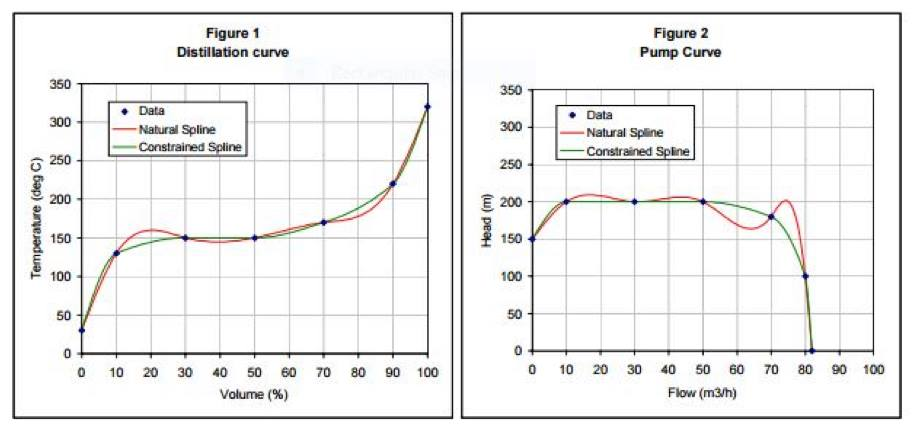
\includegraphics[width=12cm]{SplineChimie.png}
	\caption{Spline Restreintes}
\end{figure}

Les deux graphiques ci-dessus montrent les courbes obtenues \`a travers l'interpolation par splines cubiques restreintes ou non entre 7 points. Pour la distillation ainsi que pour la pompe, on remarque une assez nette diff\'{e}rence entre ces deux courbes : les splines restreintes varient bien moins ! On peut donc voir que m\^{e}me si elle peut s'av\'{e}rer tr\`{e}s pratique, la m\'{e}thode d'interpolation par splines cubiques n'est pas optimale pour toutes les applications et peut \^{e}tre am\'{e}lior\'{e}e dans certains domaines.

\newpage
\begin{huge}
\subsection{Les splines et l'imagerie m\'edicale}
\end{huge}

Nous avons vu que l'industrie regorge de domaines d'application pour les splines. Il ne faut cependant pas en conclure qu'il s'agit des seules applications possibles des splines ! Certains chercheurs essayent en effet de faire valoir les avantages des splines dans le domaine de l'imagerie m\'{e}dicale. L'Ecole Polytechnique F\'{e}d\'{e}rale de Lausanne (Suisse) se trouve au premier plan de cette bataille. Elle comporte un groupe de recherche entier baptis\'{e} Biomedical Imaging Group (BIG) qui fait beaucoup de z\`{e}le dans cette direction.

Nous citerons particuli\`erement E. Meijering et M.Unser qui ont publi\'{e} un grand nombre d'articles et de publications. Les chercheurs du BIG consid\`{e}rent en effet que les splines pr\'{e}sentent le meilleur rapport \guillemotleft \ temps de calcul/prix \guillemotright \ de toutes les m\'{e}thodes d'interpolation, ce qui les rend id\'{e}ales dans un domaine o\`u le traitement du signal est aussi important que l'imagerie m\'{e}dicale.

\newpage
\begin{huge}
\subsection{Application de splines : le Taj Mahal}
\end{huge}

Afin de voir par nous-m\^{e}me la fid\'{e}lit\'{e} de mod\'{e}lisation des splines, nous avons d\'{e}cid\'{e} de mod\'{e}liser une courbe en 2D : une image du Taj Mahal. A l'aide du logiciel Gimp, nous avons pris les coordonn\'{e}es de quelques points du contour de la structure sur l'image d'origine puis nous avons utilis\'{e} le logiciel Geogebra pour mod\'{e}liser les splines obtenus entre ces points.

\begin{figure}[h]
	\centering
	\includegraphics[width=10cm]{TajMahal.jpeg}
	\caption{Photo du Taj Mahal}
\end{figure}

\begin{figure}[h]
	\centering
	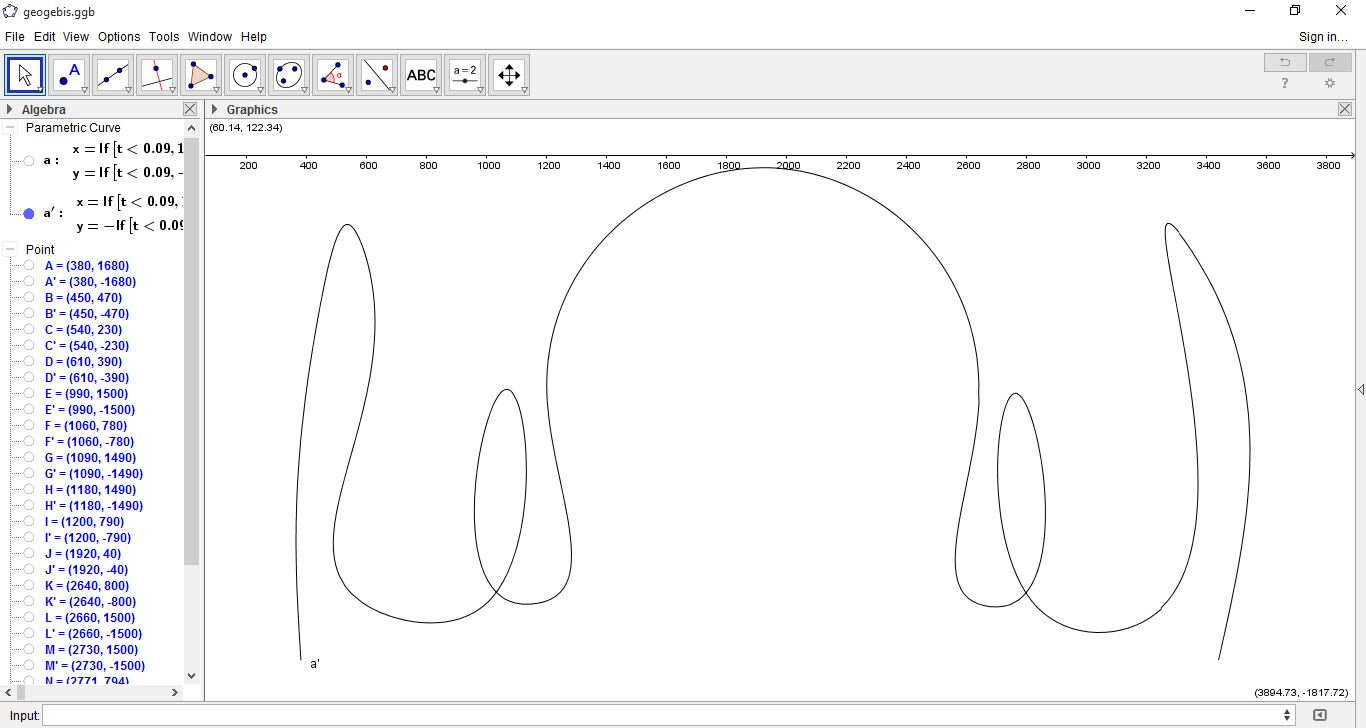
\includegraphics[width=10cm]{GeogebraTajMahal.JPG}
	\caption{Mod\'elisation du Taj Mahal par splines cubiques sur Geogebra}
\end{figure}

On remarque que m\^{e}me si les contours de l'image obtenue ont tendance \`a \^{e}tre plus courb\'{e}s que sur l'image originale, la structure du Taj Mahal reste reconnaissable. Le manque de pr\'{e}cision vient aussi du nombre de points \`a interpoler: nous en avons pris 20, mais en rajoutant des points, les d\'{e}tails de la structure commenceront \`a appara\^itre.

\newpage
\section{Conclusion}

\indent
Apr\`{e}s avoir retrac\'{e} l'histoire de l'interpolation, nous avons approfondi, dans l'ordre chronologique, les diff\'{e}rentes m\'{e}thodes : tout d'abord les courbes de B\'{e}zier puis les splines cubiques pour ensuite finir avec les B-Splines. Pour chaque technique d'interpolation, nous avons pr\'{e}sent\'{e} le contexte, d\'{e}velopp\'{e} la r\'{e}solution math\'{e}matiques et informatique et expliqu\'{e} les avantages et inconv\'{e}nients. S'ensuit des exemples de fonctions construites par splines cubiques. Nous avons achev\'{e} notre rapport par la pr\'{e}sentation d'applications possibles de cette m\'{e}thode. Notons que les exemples et applications expos\'{e}s dans notre travail ne repr\'{e}sentent qu'un petit \'{e}chantillon de la r\'{e}alit\'{e}.
\

Nous avons aim\'{e} travailler sur ce sujet. En effet, ce projet nous a permis d'explorer la m\'{e}thode d'interpolation par splines cubiques qui nous \'{e}tait auparavant m\'{e}connue. La compr\'{e}hension math\'{e}matiques de l'interpolation par splines cubiques est complexe mais apr\`{e}s de nombreuses recherches, manipulations du programme et calculs de splines, nous avons r\'{e}ussi \`{a} aboutir \`{a} un travail int\'{e}ressant et enrichissant.
\

	Nous avons ainsi pu nous rendre compte de l'utilit\'{e} et de l'importance de cette m\'{e}thode dans de nombreux domaines d'applications non seulement en math\'{e}matiques mais aussi en a\'{e}ronautique, chimie, typographie, etc. Comme nous l'avons vu, les courbes de B\'{e}zier sont la base de l'interpolation par splines cubiques qui a ensuite \'{e}volu\'{e} vers les B-splines : ce proc\'{e}d\'{e} est en constante \'{e}volution.  Bref, l'actualit\'{e} de ce domaine est tr\`{e}s grande : les courbes et les surfaces d'interpolation et d'approximation sont utilis\'{e}es partout. Il suffit de choisir un objet au hasard, il est probable qu'une des notions \'{e}tudi\'{e}es dans notre travail ait \'{e}t\'{e} utilis\'{e}es.
\

	Nous avons de plus d\'{e}couvert le langage LaTex qui est tr\`{e}s utilis\'{e} pour l'\'{e}criture de documents scientifiques ainsi que r\'{e}utilis\'{e} des logiciels de mod\'{e}lisation g\'{e}om\'{e}trique comme Geogebra. Un certain temps a \'{e}t\'{e} n\'{e}cessaire afin de comprendre et s'approprier ce langage mais la connaissance du logiciel Texmaker nous sera tr\`{e}s probablement utile pour l'\'{e}laboration d'autres documents scientifiques.

\newpage
\section{Cr\'{e}dits d'illustration}

\begingroup\raggedleft
\textbf{Figure 1} - Ancienne table de pierre.
\endgroup
\\Source : \url{https://imagescience.org/meijering/research/chronology/}
\\
\\
\textbf{Figure 2} - Ducks.
\\Source : \url{http://www.duckworksmagazine.com/03/r/articles/splineducks/splineDucks.htm}
\\
\\
\textbf{Figure 3} - Pierre B\'ezier, 1958.
\\Source : \url{http://www.fondam.org/Portraits/PierreBezier}
\\
\\
\textbf{Figure 4} - Renault 4CV.
\\Source :\url{https://quatrecylindres.com/2010/12/08/dans-le-retro-de-}
\\\url{pierre-hugonnaud-renault-4cv-la-puce-de-billancourt/}
\\
\\
\textbf{Figure 5} - Exemple d'interpolation par spline cubique sur Geogebra.
\\
\\
\textbf{Figure 6} - Analyse descendante du prgramme.
\\
\\
\textbf{Figure 7} - Courbe de B-spline de degr\'e 3.
\\Source : \url{http://www.sens-neuchatel.ch/bulletin/no34/art3-34.pdf}
\\
\\
\textbf{Figure 8} - Analyse descendante du programme.
\\
\\
\textbf{Figure 9} - Tableau de r\'esultats de la fonction de Runge en fonction des valeurs de x.
\\
\\
\textbf{Figure 10} - Repr\'esentation graphique de la fonction de Runge sur l'intervalle $[-1;1]$.
\\
\\
\textbf{Figure 11} - Repr\'esentation graphique de l'interpolation de la fonction de Runge par spline cubique.
\\
\\
\textbf{Figure 12} - Repr\'esentation graphique du ph\'enom\`ene de Runge visible aux extr\'emit\'es de l'intervalle de d\'efinition.
\\Source : \url{http://johan.mathieu.free.fr/maths/doc_maths/oral_1_capes/phenomene_Runge_projet_licence.pdf}
\\
\\
\textbf{Figure 13} - Mod\'elisation de la fonction Cosinus par spline cubique.
\\
\\
\textbf{Figure 14} - Repr\'esentation graphique de la fonction exponentielle sur l'intervalle $[-1;3]$.
\\
\\
\textbf{Figure 15} - Nouvelle repr\'esentation graphique de la fonction exponentielle sur l'intervalle $[-1;3]$ avec Geogebra.
\\
\\
\textbf{Figure 16} - La lettre e avec un ordinateur des ann\'ees 80 (gauche) et un ordinateur d'aujourd'hui (droite).
\\Source : \url{BezierDP.pdf}
\\
\\
\textbf{Figure 17} - Dessin (\`a l'aide de B-splines) r\'ealis\'e par ordinateur avec le logiciel Geogebra. 
\\Source : \url{BezierDP.pdf}
\\
\\
\textbf{Figure 18} - Ing\'enieur chez Boeing. 
\\Source : \url{http://www.boeingimages.com/archive/Engineer-Drafting-with-}
\\\url{a-Physical-Spline-2F3XC5LBLBL.html}
\\
\\
\textbf{Figure 19} - Splines restreintes. 
\\Source : \url{ http://www.korf.co.uk/spline.pdf}
\\
\\
\textbf{Figure 20} - Photo du Taj Mahal.
\\Source : \url{http://img0.svstatic.com/wallpapers/7516c8b89bf97f0219f074a}
\\\url{24515b7c9-large.jpeg}
\\
\\
\textbf{Figure 21} - Mod\'elisation du Taj Mahal par splines cubiques sur Geogebra.

\newpage
\section{Bibliograpie}

Sources que nous avons utilis\'{e} pour d\'{e}velopper le rapport :
\\
{\color{blue}
\url{https://patrimoine.gadz.org/gadz/bezier.htm}}
\\\\
{\color{blue}
\url{http://www-groups.dcs.st-and.ac.uk/history/Biographies/Schoenberg.html}}
\\\\
{\color{blue}
\url{http://www.sens-neuchatel.ch/bulletin/no34/art3-34.pdf}}
\\\\
{\color{blue}
\url{http://www.math.u-psud.fr/~perrin/CAPES/geometrie/BezierDP.pdf}}
\\\\
{\color{blue}
\url{https://en.wikipedia.org/wiki/B-spline}}
\\\\
{\color{blue}
\url{https://fr.wikipedia.org/wiki/Spline#Spline_serr.C3.A9e}}
\\\\
{\color{blue}
\url{https://en.wikipedia.org/wiki/Spline_(mathematics)#History}}
\\\\
{\color{blue}
\url{http://bigwww.epfl.ch/publications/meijering0201.pdf}}
\\\\
{\color{blue}
\url{https://fr.wikipedia.org/wiki/Interpolation_num%C3%A9rique}}
\\\\
{\color{blue}
\url{http://bigwww.epfl.ch/publications/meijering0201.pdf}}
\\\\
{\color{blue}
\url{http://www.math.univ-toulouse.fr/~cnegules/Article/beziers.pdf}}
\\\\
{\color{blue}
\url{https://fr.wikipedia.org/wiki/Courbe_de_B%C3%A9zier}}
\\\\
{\color{blue}
\url{https://imagescience.org/meijering/research/chronology/}}
\\\\
{\color{blue}
\url{https://www.math.u-bordeaux.fr/~pfischer/Teaching_files/cours.pdf}} (page 8 et 9)
\\\\
{\color{blue}
\url{https://www.youtube.com/watch?v=kF-75RRvCbs}} 
\\\\
{\color{blue}
\url{http://www.labri.fr/perso/schlick/simg/cours10.pdf}}
\\\\
{\color{blue}
\url{http://pulsar.webshaker.net/2012/08/29/les-courbes-de-bezier-1/}}
\\\\
{\color{blue}
\url{http://perso.univ-lyon1.fr/jean-claude.iehl/Public/educ/ENS/chap6_Courbes.pdf}}
\\\\
{\color{blue}
\url{http://ccmuzzo.free.fr/perso/projets/Splines.pdf}}
\\\\
{\color{blue}
\url{http://www.giref.ulaval.ca/~afortin/mat17442/documents/splines.pdf}}
\\\\
{\color{blue}
\url{http://homepages.ulb.ac.be/~majansen/teaching/INFO-F-205/diapositives05interpolation_4.pdf}}
\\\\
{\color{blue}
\url{http://www.math.univ-metz.fr/~croisil/M1-0809/2}}
\\\\
{\color{blue}
\url{https://fr.wikipedia.org/wiki/NURBS}}
\\\\
{\color{blue}
\url{https://fr.wikipedia.org/wiki/Spline}}
\\\\
{\color{blue}
\url{http://johan.mathieu.free.fr/maths/doc_maths/oral_1_capes/phenomene_Runge_projet_licence.pdf}}
\\\\
{\color{blue}
\url{http://w3.bretagne.ens-cachan.fr/math/people/gregory.vial/files/cs/interp.pdf}}
\\\\
Pour l'\'{e}criture du rapport avec Texmaker :
\\
{\color{blue}
\url{http://tex.stackexchange.com/}}

\end{document}